% ========================================= TEMPLATE INFO ========================================
%
% Author:       P4ntomime
% Version:      1.0.0
% Last updated: 2024-02-18
% Brief:        A LaTeX template for summaries. See README.md for more information.
% 
% ================================================================================================
\documentclass[8pt, a4paper, twoside]{extarticle}
% Font size:    8pt
% Paper size:   A4
% style:        twoside (needed, so odd and even pages have different margins)
% orientation:  portrait. (use 'landscape' for landscape orientation)


% ========================================= DOCUMENT INFO =========================================
\def\title{Funktionen mehrerer Variablen}                               % title
\def\shorttitle{FuVar}                                                  % short title (displayed as PDF title)
\def\dozent{Prof. Dr. Bernhard Zgraggen}                                % lecturer
\def\semester{FS 2024}                                                  % semester
\def\author{Laurin Heitzer, Flurin Brechbühler}                         % author(s)
\def\repo{https://github.com/P4ntomime/funktionen-mehrerer-variablen}   % repository link
\def\version{0.1.\today}                                                % version
\def\pagelimit{12}                                                      % page limit -> causes pages after limit to be red


% ================================= PACKAGES, SETUP AND COMMANDS ==================================
\input{preamble.tex}

% =========================================== DOCUMENT ============================================
\begin{document}
    \begin{layout}
        \section{Dimensionen, Schnitte und Konturen}

\subsection{Dimensionen}

$$f: \mathbb{D}_f (\subseteqq  \rreal^{\cbl{\bm{m}}}) \longrightarrow \mathbb{W}_f (\subseteqq  \rreal^{\cgn{\bm{n}}})$$


\begin{ctabular}{O l}
    \cbl{\bm{m}}    & Anzahl Dimensionen von ${\mathbb{D}_f}$, wobei $\cbl{\bm{m}}$ ${\in \nnatural }$\\
    \cgn{\bm{n}}    & Anzahl Dimensionen von ${\mathbb{W}_f}$, wobei $\cgn{\bm{n}}$ ${\in \nnatural }$\\
    \vec{f}         & wenn Output vektoriell
\end{ctabular}

\warn{Variablen sind abhängig von einander!}


\subsubsection*{Multi-Variat:}

Die Funktion ${f}$ ist "Multi-Variat", wenn:
\begin{itemize}
    \item Input, Output oder beides mehrdimensional ist.\\
    (Nur wenn Input \textbf{und} Output Skalare sind ist eine Funktion nicht Multi-Variat.)
\end{itemize}
%\example{Multi-Variat}
%\begin{ctabular}{O l}
%    (x;y) \mapsto \text{Skalar} \Rightarrow \text{Multi-Variat}\\
%    (x;y;z) \mapsto \text{Skalar} \Rightarrow \text{Multi-Variat}\\
%    (t;x;y;z) \mapsto \text{Skalar} \Rightarrow \text{Multi-Variat}\\
%\end{ctabular}


\subsubsection{Raumzeit}

$$\left.\begin{array}{r@{}}
    \text{Raum 3D ${(x;y;z)}$ }\rreal^3\\
    \text{Zeit 1D ${(t)}$ }\rreal^1
\end{array}\right\rbrace \rreal^{1}\times \rreal^3 (t;x;y;z) = \text{4D Raumzeit}$$


\subsubsection{Stationärer Fall}
$${t \rightarrow \infty \rightarrow \text{Stationär}}$$
$${\crd{T(x;y;z) \enspace\frac{\Delta{T}}{\Delta{t}} \rightarrow 0 }}$$


\subsubsection{Koordinatenvektoren = Einheitsvektoren}
$\vec{i}=\hat{i}=\vec{{e}_1}=
\begin{pmatrix}
    1 \\
    0 \\
    0
\end{pmatrix},\enspace
\vec{j}=\hat{j}=\vec{{e}_2}=
\begin{pmatrix}
    0 \\
    1 \\
    0
\end{pmatrix},\enspace
\vec{k}=\hat{k}=\vec{{e}_3}=
\begin{pmatrix}
    0 \\
    0 \\
    1
\end{pmatrix}$


\subsection{Schnitte}
Schnitt = Restriktion $\rightarrow$ Teilmenge vom Definitionsbereich ${\mathbb{D}_f}$


\subsubsection{Partielle Funktion}

\begin{itemize}
    \item Nur \textbf{eine} Variable ist frei! (wählbar)
    \item \textbf{Alle} anderen Variablen sind fix!
    \item[] \warn{$\mathbb{W}_f$ Analyse!}
\end{itemize}


\subsection{Konturen, Levelsets, Niveaulinien, ...}
Output = konstant = const. = fix: 
$$\vec{y} = \vec{f}(\vec{x}) = \text{const. wobei } \vec{x} \subset \mathbb{D}_f$$
Man spricht von "Konturen, Levelsets oder Niveaulinien",\\
wenn der Output von ${f}$ konstant ist.\\
\crd{Hier wäre ein Bild von Höhenlinien aus dem Skript cool}


        \newpage
\section{Ableitungen, DGL und Gradienten (bi-variat)}
\[
    f:\mathbb{D}_f\subseteq \mathbb{R}^2\rightarrow \mathbb{W}_f\subseteq \mathbb{R}\quad\mathrm{skalar}
\]
\subsection{Partielle Ableitung}
Ableitung einer Partiellen Funktion. 

\example{Bi-Variate Funktion}
\[
    f(x, y):\, y \text{ fixieren} = \text{const.} = y_{0};\quad x \text{ \textbf{einzige} freie Variable}
\]

\subsubsection*{Notationen}

\begin{ctabular}{l l}
    1. Ordnung: & $\displaystyle f(x; y_{0})\Rightarrow \frac{\partial f}{\partial x} = f_{x}(x; y_{0})$ \\
    \multirow{2}*{2. Ordnung:}  &  $\displaystyle \frac{\partial}{\partial x}
                                    \left\lgroup\frac{\partial f}{\partial x}\right\rgroup = 
                                    \frac{\partial^{2}f}{\partial x^{2}} = f_{xx}$\\
                                &  $\displaystyle \frac{\partial}{\partial y}
                                        \left\lgroup\frac{\partial f}{\partial x}\right\rgroup = 
                                    \frac{\partial^{2}f}{\partial y \partial x} = f_{xy}$
\end{ctabular}


\subsubsection{Schwarz-Symmetrie}
Wenn \cor{$f_{xx}, f_{yy}, f_{xy}$ \& $f_{yx}$} \textbf{stetig} (sprungfrei) sind, dann gilt:
\[
    f_{xy} \overset{!}{=} f_{yx}
\]

         
\subsection{Gradient (Nabla-Operator)}
Spaltenvektor mit partiellen Ableitungen
\[
    \tikznode{grad}{\nabla} f = \begin{pmatrix}
        \frac{\partial f^{\mathstrut}}{\partial^{\mathstrut} x}\\
        \frac{\partial f^{\mathstrut}}{\partial^{\mathstrut} y}\\
        \vdots      % TODO: reformat vdots. They look like shit
    \end{pmatrix} \hat{=} \text{Vektorfeld}
\]

% TODO: some TikZ. Might not be needed and could be removed if unnecessary
\begin{tikzpicture}[overlay, remember picture, >={Latex}]
    \node[inner sep=0pt, ellipse, fit=(grad), draw, densely dotted]{};
    \node[below left= 2mm and 5mm of grad] (gtext) {\txtqt{Gradient} / Nabla};
    \draw[->, rounded corners] (gtext.east) -| ($(grad.south)+(0,-1mm)$);
\end{tikzpicture}


\subsection{Totale Ableitung}
Für Fehlerrechnung benützt, da man hierbei die Abstände von $(x; y; z)$ 
zu einem festen Punkt $(x_{0}; y_{0}; z_{0})$ erhält. (relative Koordinaten)

\[
    D(f;\underbrace{(x_{0}, y_{0}, \ldots)}_{\text{Arbeitspunkt}}):\, 
    \rreal^{\tikznode{somea}{\scriptstyle 2}} \rightarrow \rreal^{\tikznode{someb}{\scriptstyle 1}};\, 
    \text{\txtqt{gute Approximation}}
\]
\[
    f(x = x_{0} + \Delta x; y = y_{0} + \Delta y; \ldots) = (D_{11}; D_{12})\cdot \begin{pmatrix}
        \Delta x\\
        \Delta y
    \end{pmatrix} + f(x_{0}; y_{0}) + \cgn{R_{1}}
\]
Wobei \cgn{$R_{1}$} dem \txtqt{Rest} entspricht. (Ähnlich wie bei Taylorreihe)

\begin{minipage}[c]{0.7\columnwidth}
    \[
        \frac{\cgn{R_{1}}}{\cor{d = \sqrt{\Delta x^{2} + \Delta y^{2}}}} \rightarrow 0 \text{ (\txtqt{gut}, \txtqt{schneller gegen 0 als $\cor{d}$})}
    \]
\end{minipage}\hfill
\begin{minipage}[c]{0.29\columnwidth}
    \begin{tikzpicture}[baseline=(current bounding box.center), 
                        >={Latex[width=1mm, 
                                 length=1mm]}, 
                        scale=0.5, 
                        font=\tiny]

        % Koordinatensystem
        \draw[->] (0,0) -- (4,0) node[below]{$x$};
        \draw[->] (0,0) -- (0,2.5) node[left]{$y$};

        % Punkte
        \node[circle, fill=black, inner sep=0pt, minimum size=2pt] (A) at (1.7,0.7) {};
        \node[circle, fill=black, inner sep=0pt, minimum size=2pt] (P) at (0.7,1.7) {};
        \node[inner sep=1pt, right=1mm of A] {$A=(x_{0}; y_{0})$};
        \node[inner sep=1pt, above right=0.1mm and -1ex of P] {$P=(x;y)$};
    
        % Differenz
        \draw (P) -- (A-|P) node[midway, left]{$\Delta y$} -- (A) node[midway, below]{$\Delta x$};
        \draw[orange] (P) -- (A) node[midway, above right, inner sep=1pt]{\cor{$d$}};
    \end{tikzpicture}
\end{minipage}

\[
    \begin{split}
        D(f;(x_{0}; y_{0})) &= \left\lgroup D_{11} = \frac{\partial f}{\partial x}(x_{0}; y_{0}); 
                                            D_{12} = \frac{\partial f}{\partial y}(x_{0}; y_{0})\right\rgroup\\
        &= (\nabla f)^{\tr} \text{ \cbl{wenn $\frac{\partial f}{\partial x}; \frac{\partial f}{\partial y}$ stetig bei $A$}}
    \end{split}
\]

\begin{tikzpicture}[overlay, remember picture]
    \draw[tips, -{Latex}] (someb) to[out=135, in=45, edge node={node[above=0mm]{\tiny $1\times 2$ Matrix}}] (somea);
\end{tikzpicture}


\subsection{Linearapproximation (Tangentialapproximation)}
\[
    f(x;y) \approx f(x_{0}; y_{0}) + D(f;(x_{0}; y_{0}))\cdot \begin{pmatrix}
        \Delta x\\
        \Delta y
    \end{pmatrix}
    \quad\text{ linear in $\Delta x$ und $\Delta y$}
\]


\subsubsection{Tangentialebene}
\[
    \crd{g(x; y) = f(x_{0}; y_{0}) + D(f;(x_{0}; y_{0}))\cdot \begin{pmatrix}
        x - x_{0}\\
        y - y_{0}
    \end{pmatrix}}
\]
\[
    g(x;y)=f(x_0;y_0)+f_x(x_0;y_0)\cdot(x-x_0)+f_y(x_0;y_0)\cdot(y-y_0)
\]

\subsubsection{Tangentialer Anstieg (Totale Differential)}
\[
    \cvt{\diff f \overset{!}{=} 
        \frac{\partial f}{\partial \tikznode{ptx}{x}}\diff x + 
        \frac{\partial f}{\partial \tikznode{pty}{y}}\diff y} 
        \quad \text{bezüglich } A=\underbrace{(x_{0}; y_{0})}_{\tikznode{axy}{}}
\]
\begin{tikzpicture}[overlay, 
                    remember picture, 
                    >={Latex[width=1mm, 
                             length=1mm]}]

    \draw[->] ($(axy)+(0, 1.8mm)$) to[bend left=10] (ptx.south east);
    \draw[->] ($(axy)+(0, 1.8mm)$) to[bend left=10] (pty.south east);
\end{tikzpicture}


\subsubsection{Differential-Trick (\texorpdfstring{$\diff f$}{df} Trick)}
\begin{minipage}[c]{0.5\columnwidth}
    \[\left\lgroup\begin{aligned}
        f &= c = \mathrm{const.} \quad | \diff(\ldots)\\
        \diff f &= \diff c \overset{!}{=} 0
    \end{aligned}\right\rgroup\]
\end{minipage}\hfill
\begin{minipage}[c]{0.5\columnwidth}
    \[
        f_{x}\diff x + f_{y}\diff y = 0 \quad \text{für Kontourlinien}
    \]
\end{minipage}


\subsubsection{Implizite (Steigungs-)Funktion}
\begin{minipage}[c]{0.6\columnwidth}
    \[
        \cbl{y'(x)} = \frac{\diff y}{\diff x} = -\frac{f_{x}}{f_{y}\crd{\neq 0}} \lor 
        \cbl{x'(y)} = \frac{\diff x}{\diff y} = -\frac{f_{y}}{f_{x}\crd{\neq 0}}
    \]
\end{minipage}\hfill
\begin{minipage}[c]{0.39\columnwidth}
    \begin{tikzpicture}[>={Latex[width=1mm,
                                 length=1mm]}, 
                        scale=0.75, 
                        font=\small]

        % Koordinatensystem
        \draw[->] (0,0) -- (3,0) node[below]{$x$};
        \draw[->] (0,0) -- (0,2) node[left]{$y$};
        
        % Funktionen
        \draw[color=green] plot[domain=0.55:1.5] (\x, {-((\x-1.5)*(\x-1.5))+1}) node[right]{$y$}; % y = -((x-1.5)^2)+1
        \draw[color=blue] node[above right]{$y'$} plot[domain=0.25:1.5] (\x, {\x-0.25}); % y = x-0.25

        % Arbeitspunkt
        \node[circle, fill=black, inner sep=0pt, minimum size=1.5pt] (P) at (1,0.75) {};
        \node[inner sep=0pt, above left=0.25mm and 0mm of P] {$P_{0}$};
        \draw[gray, dashed] (P) -- (P-|0,0) node[left]{$y_{0}$};
        \draw[gray, dashed] (P) -- (P|-0,0) node[below]{$x_{0}$};

        % Richtungselemente
        \draw[orange, semithick, ->] (P) -- (2,1.75) node[above, midway, rotate=45]{$\vec{r}$};
        \draw[->] (P) -- (P-|2,0) node[midway, below]{$\diff x$};
        \draw[->] (P-|2,0) -- (2,1.75) node[midway, right]{$\diff y$};
    \end{tikzpicture}
\end{minipage}




% \subsection{Differential}


\subsection{DGL}
\[
    y' = \tikznode{rhsfn}{\bbr{violet}{-\frac{f_{x}}{f_{y}}}};\, y(x_{0}) = y_{0}
\]
\begin{tikzpicture}[overlay, 
                    remember picture] 
    \node[below=1mm of rhsfn, inner sep=0pt, font=\tiny, text=violet] {right-hand-side (r.h.s.) Funktion};
\end{tikzpicture}


\subsection{Richtungselement (Tangentiallinie an Kontouren)}
\[
    \vec{r} = \left\lgroup\diff x = h; \diff y = y'\diff x = -\frac{f_{x}}{f_{y}}\diff x\right\rgroup^{\tr}
\]


\subsection{Gradientenfeld \texorpdfstring{$\perp$}{\_|\_} Kontouren}
\[
    \nabla f \tikznode{scprd}{\dotp} \begin{pmatrix}
        \diff x\\
        \diff y = y'\diff x
    \end{pmatrix} \overset{!}{=} 0
\]
\begin{tikzpicture}[overlay,
                    remember picture,
                    >={Latex[width=1mm, 
                             length=1mm]}]
    \node[above left=2mm and 4mm of scprd, inner sep=0pt, anchor=south east] (spnode) {Skalarprodukt};
    \draw[->] (spnode.east) to[out=0, in=90] ($(scprd.north)+(0,0.2mm)$);
\end{tikzpicture}


\subsection{?Wie heisst dieser Abschnitt?}

\begin{tikzpicture}[>={Latex[width=1mm,
                       length=1mm]}]
    \draw[->] (-1,0) -- (3,0) node[below]{$x$};
    \draw[->] (0,-0.5) -- (0,2) node[left]{$y$};

    % Schnitt
    \draw[green] (-1,-0.5) -- (1, 0.75);
\end{tikzpicture}


\begin{ctabular}{r l}
    $s(t) :$    &$P_0 + t \cdot \hat{v} \mid t\in \rreal$\\
    $s(t) :$    &$f(x_0 + t \cdot \hat{v}_1\, ;\, y_0 + t \cdot \hat{v}_2)$\\
    &\\
    $\frac{\diff s(t)}{\diff t}=\dot{s}(t) :$&$t\mapsto\overbrace{\begin{pmatrix}x_0+t\cdot v_1\\y_0+t\cdot v_2\end{pmatrix}}^{\begin{pmatrix}x\\y\end{pmatrix}}\mapsto f(x,y)$
\end{ctabular}


\subsection{Richtungs-Ableitung}
\[
    \frac{\partial f}{\partial\hat{v}}\overset{!}=D(f;(x_{0};y_{0}))\cdot\hat{v}\overset{\text{Def.}}\Leftrightarrow \grad(f)^{\tr}\cdot\hat{v}=f_{x}\cdot v_{1}+f_{y}\cdot v_{2}
\]

\example{Richtungs-Ableitung}

\[
    \vec{x} : \vec{v} = 
\begin{pmatrix}
    1\\
    0
\end{pmatrix}
= \hat{e}_1
\quad\Rightarrow\quad
    \frac{\partial f}{\partial\hat{e}_{1}}=f_{x}\cdot1+f_{y}\cdot0=\uuline{f_{x}\strut}
\]


\subsubsection{Spezialfälle}


\begin{minipage}[c]{.72\columnwidth}
    \begin{outline}
        \1 $\alpha = \frac{\pi}{2}$ \textrightarrow\ rechter Winkel % TODO: fix \pi --> should be upright
        \1 $\frac{\partial f}{\partial \hat{v}}$ extremal
            \2 $\alpha = 0$ (max):   $\nabla f \cdot\hat{v} > 0$ \textrightarrow\ \cbl{$\grad(f)$} liegt auf $\hat{v}$
            \2 $\alpha = \pi$ (min): $\nabla f \cdot\hat{v} < 0$ \textrightarrow\ \cbl{$\grad(f)$} liegt invers auf $\hat{v}$
    \end{outline}
\end{minipage}\hfill
\begin{tikzpicture}[%
    baseline=(current bounding box.center),
    scale=0.75,
    >={Latex[%
        width=1mm, 
        length=1mm]}]
    \coordinate (A) at (0,0);
    \coordinate (B1) at (2,0);
    \coordinate (B2) at (2.4,0);
    \coordinate (C) at (2,0.8);

    \draw[->] (A) -- (B2) node[right]{$\hat{v}$};
    \draw[blue, ->] (A) -- (C) node[above=-1mm]{$\grad(f)$};
    \draw[red, ->] (A) -- (B1) node[midway, below]{$\nabla f \dotp \hat{v}$};

    \draw[gray, densely dashed] (C) -- (B1);

    \draw pic[draw=green, angle radius=10mm, pic text=$\alpha$, pic text options=green] {angle=B1--A--C};
    \draw pic[draw=gray, angle radius=2mm, pic text=. , pic text options=gray] {angle=C--B1--A};

    \fill (A) circle (1pt) node[above]{$P_0$};
\end{tikzpicture}

\para{Trigo} $\nabla f\cdot\hat{v} \land \frac{\partial f}{\partial\hat{v}}$ \textrightarrow\ $\cos(\alpha)\cdot\abs{\cbl{\nabla f}}$


        % TODO: Taylorreihe
        
        \newpage
\section{Extrema von Funktionen zweier Variabeln finden}

\begin{enumerate}[itemsep=1ex]
    \item \textbf{Gradient von $f$ Null-setzten und kritische Stellen finden:}

    $\nabla f=
    \begin{pmatrix}
        f_x\\
        f_y
    \end{pmatrix} \stackrel{!}{=}
    \begin{pmatrix}
        0\\
        0
    \end{pmatrix}
    \, \, \, \, \, \,
    \Rightarrow 
    \begin{matrix}
        f_{x}=0\\
        f_{y}=0
    \end{matrix}
    \, \, \, \, \, \,
    \Rightarrow
    x_0 \text{ und } y_0 \text{ bestimmen}$

    \item \textbf{Zweite Partielle Ableitungen bestimmen:}
    
    $\begin{aligned}
        f_{xx} &= \dots\\
        f_{xy} &= f_{yx} = \dots\\
        f_{yy} &= \dots
    \end{aligned}$
    

    \item \textbf{Determinante $\Delta$ der Hesse-Matrix H bestimmen:}
    
    $\Delta = f_{xx}(x_0;y_0) \cdot f_{yy}(x_0;y_0) - \left(f_{xy}(x_0;y_0)\right)^2 $

    \item \textbf{Auswertung:}
    
    \begin{tabular}{lllcl}
        \hline
        $\Delta > 0$ &AND& $f_{xx}(x_0;y_0) < 0$ &$\Longrightarrow$& $\text{lokales Maximum}$\\
        \hline
        $\Delta > 0$ &AND& $f_{yy}(x_0;y_0) < 0$ &$\Longrightarrow$& $\text{lokales Maximum}$\\
        \hline
        $\Delta > 0$ &AND& $f_{xx}(x_0;y_0) > 0$ &$\Longrightarrow$& $\text{lokales Minimum}$\\
        \hline
        $\Delta > 0$ &AND& $f_{yy}(x_0;y_0) > 0$ &$\Longrightarrow$& $\text{lokales Minimum}$\\
        \hline
        $\Delta < 0$ &&&$\Longrightarrow$& $\text{Sattelpunkt}$\\
        \hline
        $\Delta = 0$ &&&?& $\text{Multi-variate-Taylor-logik ...}$\\
        \hline
    \end{tabular}

\end{enumerate}


        \newpage
\section{Support Vector Machine (SVM)}
Die Support Vector Machine kann verwendet werden, um ein Modell für das Zuordnen von Daten zu entwickeln.
Dadurch wird ein Satz von Punkten, deren Klassifizierung bekannt ist, so linear getrennt, dass der Abstand von der trennenden Geraden zu den beiden Punktegruppen maximal wird.
Es resultiert eine einfache Gleichung, mit der sich neue Daten klassifizieren lassen.

\subsection{Linear Trennbare Daten}
\subsubsection{Allgemeines}

\myul{\textbf{Datenpunkte:}} (2D Beispiel)\\
\begin{tabular}{lllll}
    $A:(\underbrace{(x_1,x_2)}_{\vec{x}_1};y_1)$, &
    $B:(\underbrace{(x_1,x_2)}_{\vec{x}_2};y_2)$, &
    $C:(\underbrace{(x_1,x_2)}_{\vec{x}_3};y_3)$, & 
    $\cdots $, &
    $N:(\underbrace{(x_1,x_2)}_{\vec{x}_n};y_n)$\\
\end{tabular}

$\vec{x}_j$ sind Datenvektoren\\
$y_j$ $\in $ \{$\pm 1$\} klassifiziert die jeweiligen Datenvektoren
\newline
\begin{minipage}[]{0.56\columnwidth}
    \myul{\textbf{Hyperebenen:}}\\
    $\boxed{\vec{w}^{tr}\cdot\vec{x}+b=0}$ \\
    $\vec{w}$: Normalenvektor, $\vec{w} \in \mathbb{R}^d$ und $\vec{w} \neq 0$\\
    $b$: Konstante, $b \in \mathbb{R}$\\
    Dimmension der Hyperebene $= d-1$\\
    Abstand der Hyperebene zum Ursprung: $\frac{\left\lvert b \right\rvert }{\left\lvert \vec{w}\right\rvert }$
    \medskip

    \myul{\textbf{Klassifizierung:}}\\
    $\boxed{\vec{w}^{tr}\cdot\vec{x}+b>0} \Rightarrow \vec{x} $ gehört zur Klasse $y = +1$\\
    $\boxed{\vec{w}^{tr}\cdot\vec{x}+b<0} \Rightarrow \vec{x} $ gehört zur Klasse $y = -1$
    \medskip

    \myul{\textbf{Klassifizierung der Trainigsdaten:}}\\
    $\boxed{\vec{w}^{tr}\cdot\vec{x}_j+b \geq 0} \Rightarrow \vec{x}_j $ gehört zur Klasse $y = +1$\\
    $\boxed{\vec{w}^{tr}\cdot\vec{x}_j+b\leq 0} \Rightarrow \vec{x}_j $ gehört zur Klasse $y = -1$
    \medskip

    \myul{\textbf{Zielfunktion:}}\\
    $\boxed{\frac{2}{\left\lvert \vec{w}\right\rvert }=\frac{2}{w}}$
\end{minipage}\hfill
\begin{minipage}[t]{0.4\columnwidth}
    \includegraphics[width=4cm]{images/7_model_values.png}
\end{minipage}

\subsubsection{Das primale Optimierungsproblem}
$\boxed{\frac12\vec{w}^{tr}\cdot\vec{w}=\frac12\left|\vec{w}\right|^2=\frac12w^2\to\min!\quad\mathrm{s.t.}\quad\left(\vec{w}^{tr}\cdot\vec{x}_j+b\right)y_j\geq1\quad\left(j=1,\cdots,N\right)}$

\subsubsection{Das duale Optimierungsproblem}
\myul{\textbf{Nebenbedingung:}}\\
$\boxed{\underbrace{1-\left(\vec{w}^{tr}\cdot\vec{x}_j+b\right)y}_{g_j(\vec{w}^{tr},b)}\leq0\Leftrightarrow g_j(\vec{w}^{tr},b)\leq0\quad\left(j=1,\cdots,N\right)}$
\medskip

\myul{\textbf{Lagrange-Funktion:}}\\
Zusammengesetzt aus dem primalen Problem und den Nebenbedingungen.\\
\begin{tabular}{|r@{ }l|}
    \hline
    $L(\vec{w}^{tr},b,\vec{a})$ & $ =L(w_1,w_2, ...,w_d,b,\alpha_1,\alpha_2, ...,\alpha_N) $ \\
                                & $ =\frac12\vec{w}^{tr}\cdot\vec{w}+\sum_{j=1}^N\alpha_j\left(\underbrace{1-\left(\vec{w}^{tr}\cdot\vec{x}_j+b\right)y_j}_{g_j\left(\vec{w}^{tr},b\right)}\right) $ \\
    \hline
\end{tabular}
\medskip

\myul{\textbf{Stationaritätsbedingungen:}}\\
Aus der Bedingung, dass $\grad(L) = 0$ sein muss, lassen sich folgende Formeln ableiten:
$\boxed{grad_{\left\{\vec{w}^{tr},b\right\}}\left(L(\vec{w}^{tr},b,\vec{\alpha})\right)=\vec{0}} \Leftrightarrow 
\boxed{\vec{w}=\sum_{j=1}^N\alpha_jy_j\vec{x}_j} \text{ und }
\boxed{\sum_{j=1}^N\alpha_jy_j=0}$\\
%\myul{\textbf{Lagrange-Funktion mit den Dualvariablen $\alpha_j$:}}\\
%$\boxed{L(\vec{w}^{tr},b,\vec{\alpha})=\sum_{j=1}^N\alpha_j-\underbrace{\frac12\sum_{j,j'=1}^N\alpha_j\alpha_j,y_jy_j,\vec{x}_j^{tr}\cdot\vec{x}_j}_{\frac{1}{2}\vec{w}^{tr}\cdot\vec{w}}:=L(\vec{\alpha})\quad , \alpha_j\geq0}$
\myul{\textbf{Das duale Problem:}}\\
Die oben erhaltenen Summen können nun in die Lagrange-Fkt. eingesetzt werden. Daraus entsteht\\
$\boxed{L(\vec{\alpha})=\sum_{j=1}^N\alpha_j-\underbrace{\frac12\sum_{j,j'=1}^N\alpha_j\alpha_{j'} \space y_jy_{j'} \space \vec{x}_j^{tr}\cdot\vec{x}_{j'}}_{=\frac12 \vec{w}^{tr} \cdot \vec{w}}\quad\to\quad\max!\quad\mathrm{s.t.}\quad\alpha_j\geq0\wedge\sum_{j=1}^N\alpha_jy_j=0}$\\

\myul{\textbf{Vorgehen zum lösen des dualen Optimierungsproblems:}}

\begin{enumerate}
    \item \myul{\textbf{Skizze mit Datenpunkten erstellen:}} \\
    \begin{minipage}[c]{0.6\columnwidth}
        \begin{itemize}
            \item Einzelne Datenpunkte klassenweise farblich hervorheben
            \item Falls ein Datenpunkt der gleichen Klasse weit weg von den anderen ist\\
            \textrightarrow\ diesen vergessen, da sein $\alpha = 0$ sein wird
        \end{itemize}
    \end{minipage}\hfill
    \begin{minipage}[c]{0.33\columnwidth}
        \includegraphics[width=\columnwidth]{images/SVM_2.png}
    \end{minipage}
    \columnbreak
    \item \myul{\textbf{Nebenbedingungen, Es muss gelten:}}
    \begin{itemize}
        \item [\textbf{a:}] $\boxed{\alpha_j\geq0}$
        \item [\textbf{b:}] $\boxed{\sum_{j=1}^N\alpha_j \cdot y_j=0}$\\
        Nach einem $\alpha$ unstellen und anschliessend jenes $\alpha$\\(damit die Nebenbedingung miteinbezogen wird) in der Lagrange-Funktion ersetzen
    \end{itemize}
    \item \myul{\textbf{Kernel-Matrix aufstellen:}}\\
        $\boxed{K\left( \vec{x}^{\text{ $tr$}} ; \vec{x}\right) = \vec{x}^{\text{ $tr$}} \bullet \vec{x}}$\\
        \includegraphics[width=5cm]{images/kernel_matrix.png}
        \begin{itemize}
            \item Einträge sind die Ergebnisse der Skalarprodukte
        \end{itemize}
    \item \myul{\textbf{Lagrange-Funktion aufstellen:}}\\
        $\boxed{L(\vec{\alpha})=\sum_{j=1}^N\alpha_j-\frac{1}{2}\sum_{j,j'=1}^N\alpha_j \cdot \alpha_{j'} \cdot \space y_j \cdot y_{j'} \cdot \space \vec{x}_j^{\text{ $tr$}} \bullet  \vec{x}_{j'}\quad\to\quad\max!}$
        \begin{itemize}
            \item \textbf{2. b} und \textbf{3} brauchen
        \end{itemize}
    \item \myul{\textbf{Alle $\alpha$ finden durch Stationaritätsbedingung}}\\
            $\boxed{\nabla L = \vec{0}}$\\
            $\Rightarrow$ ersetztes $\alpha$ mit gefundenen $\alpha$ berechnen 
    \item \myul{\textbf{$\bm{\vec{w}}$ berechnen:}}\\
        $\boxed{\vec{w}=\sum_{j=1}^N\alpha_jy_j\vec{x}_j}$
    \item \myul{\textbf{Konstante $\mathbf{b}$ berechnen:}}\\
        Datenpunkte mit der Klasse $y = 1$ oder $y = -1$ wählen und einsetzen
        \begin{itemize}
            \item \textbf{Variante 1:} Stützvektor-Datenpunkt mit $y = +1$\\
                $\boxed{\vec{w}^{tr}\cdot\vec{x}_{...} + b = 1} \Leftrightarrow  \boxed{b = 1 -\vec{w}^{tr}\cdot\vec{x}_{...} = ...}$
            \item \textbf{Variante 2:} Stützvektor-Datenpunkt mit $y = -1$\\
                $\boxed{\vec{w}^{tr}\cdot\vec{x}_{...} + b = -1} \Leftrightarrow  \boxed{b = -1 -\vec{w}^{tr}\cdot\vec{x}_{...} = ...}$
        \end{itemize}
\end{enumerate}


\subsection{Nicht linear Trennbare Daten}
Sollte ein Datensatz von nicht linear trennbaren Datenpunkten vorliegen, so muss dieser durch eine Transformation linear trennbar gemacht werden.
Dadurch werden die Punkte oft in höhere Dimensionen gebracht.
Das Finden einer geeigneten Transformation liegt nicht im Ramen dieses Moduls.

Der einzige Unterschied zu der Methode zum linearen trennen von Datenpunkten ist dann, dass stat mit den Datenpunkten $\vec{x}_i$ mit deren durch $\varphi$ transformierten gegenstücken $\vec{\varphi}(\vec{x}_i)$ gerechnet wird.\\

\subsubsection{Transformiertes duales Optimierungsproblem}
\myul{\textbf{Nebenbedingungen, Es muss gelten:}}
    \begin{itemize}
        \item [\textbf{a:}] $\boxed{\alpha_j\geq0}$
        \item [\textbf{b:}] $\boxed{\sum_{j=1}^N\alpha_j \cdot y_j=0}$
    \end{itemize}
$\boxed{L(\vec{\alpha})=\sum_{j=1}^N\alpha_j-\frac{1}{2}\sum_{j,j'=1}^N\alpha_j \cdot \alpha_{j'} \cdot \space y_j \cdot y_{j'} \cdot \space \underbrace{\vec{z}_j^{\text{ $tr$}} \bullet  \vec{z}_{j'}}_{\text{Kernel}} \quad\to\quad\max!}$

\subsubsection{Kernelfunktionen («Kernel-Trick»)}
$\boxed{K\left( \vec{x}_j ; \vec{x}_{j'}\right) = \vec{z}_j^{\text{ $tr$}}\bullet\vec{z}_{j'}=\vec{\varphi}(\vec{x}_j) \bullet \vec{\varphi}(\vec{x}_{j'})}$

$\boxed{\vec{w}=\sum_{j=1}^N\alpha_j \cdot y_j \cdot \vec{\varphi}(\vec{x}_j)}$

$\boxed{\sum_{j=1}^N\alpha_j \cdot y_j \cdot K\Big(\vec{x}_j;\vec{x}^{\text{ *}} \Big)+b>0\Longrightarrow\vec{x}^{\text{ *}}}$ gehört zur Klasse $y = +1$\\
$\boxed{\sum_{j=1}^N\alpha_j \cdot y_j \cdot K\Big(\vec{x}_j;\vec{x}^{\text{ *}} \Big)+b<0\Longrightarrow\vec{x}^{\text{ *}}}$ gehört zur Klasse $y = -1$\\
$\vec{x}^*$ steht für Test-Daten\\\\
\textcolor{gray}{Lösungsweg: gleiches Vorgehen wie beim linearen Fall.}
        \section{Koordinatensysteme}
\subsection{2D Koordinatensysteme}
Neben den Kartesischen Koordinatensystemen kommen in zweidimensionalen Räumen auch Polare Koordinatensysteme zum Einsatz.
Die beiden Systeme können mit Hilfe der Trigonometrie in einander überführt werden.

\subsubsection{Umrechnung Kartesisch $\leftrightarrow$ Polar}
\begin{minipage}{0.29\linewidth}
    \myul{Polar zu Kartesisch}
    \[
    \begin{pmatrix}
        x \\
        y
    \end{pmatrix}
    =
    \begin{pmatrix}
        r \cdot \cos{\varphi}\\
        r \cdot \sin{\varphi}
    \end{pmatrix}
    \]
\end{minipage}
\hfill
\begin{minipage}{0.29\linewidth}
    \myul{Kartesisch zu Polar}
    \[
    \begin{pmatrix}
        r \\
        \varphi
    \end{pmatrix}
    =
    \begin{pmatrix}
        \sqrt{x^2+y^2}\\
        \tan^{-1}{\frac{y}{x}}
    \end{pmatrix}
    \]
\end{minipage}
\hfill
\begin{minipage}{0.29\linewidth}
    \begin{center}
        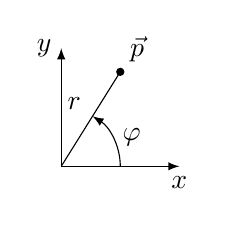
\begin{tikzpicture} [scale = 1.5]
            % Kartesische Achsen
            \draw[-{latex}] (0, 0) -- (1, 0) node [below] {$x$} ;
            \draw[-{latex}] (0, 0) -- (0, 1) node [left]  {$y$} ;

            % Punkt p
            \fill (0.5, 0.8) circle (1pt) node [anchor=south west] {$\vec{p}$};

            % Länge r
            \draw (0, 0) -- (0.5, 0.8) node [midway, above left] {$r$};
            % Winkel phi
            \draw [-{latex}] (0.5, 0) arc (0:58:0.5) node [midway, right] {$\varphi$};
        \end{tikzpicture}
    \end{center}
\end{minipage}

Dabei ist zu beachten, dass $\tan^{-1}$ nur werte von $-\frac{\pi}{2}$ bis $\frac{\pi}{2}$ liefert, für $\varphi$ jedoch $\varphi \in [0, \pi]$ gelten soll. 
$\varphi$ wird also, je nach dem in welchem Quadranten sich $\vec{p}$ befindet, nach folgendem Schema berechnet:
\begin{center}
    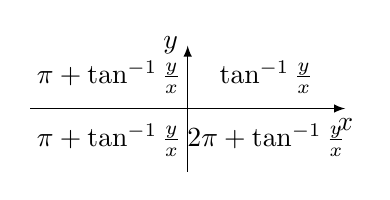
\begin{tikzpicture}
        % Achsen 
        \draw [-{latex}] (-2, 0) -- (2, 0) node [below] {$x$};
        \draw [-{latex}] (0, -0.8) -- (0, 0.8) node [left] {$y$};
        % Formeln
        \node at ( 1,  0.4) {$       \tan^{-1}\frac{y}{x}$};
        \node at ( 1, -0.4) {$2\pi + \tan^{-1}\frac{y}{x}$};
        \node at (-1, -0.4) {$\pi  + \tan^{-1}\frac{y}{x}$};
        \node at (-1,  0.4) {$\pi  + \tan^{-1}\frac{y}{x}$};
    \end{tikzpicture}
\end{center}

Um eine ganzes Integral vom einen Koordinatensystem ins andere zu überführen, muss zum einen die Funktion $ f(x, y) $ zu $ f(r, \varphi) $ (oder umgekehrt) umgeschrieben, sowie die differentiale angepasst werden.
Hier dafür einige gängige Elemente:

\begin{tabular}{l c c}
                         & \bf{Kartesisch}                   & \bf{Polar}                                                       \\
    \bf{x-Achsenelement} & $\diff x$                         & $\diff x = \cos \varphi \diff r - r \sin \varphi \diff \varphi$  \\
    \bf{y-Achsenelement} & $\diff y$                         & $\diff x = \sin \varphi \diff r + r \cos \varphi \diff \varphi$  \\
    \bf{Linienelement  } & $\diff s^2 = \diff x^2 \diff y^2$ & $\diff s^2 = \diff r^2 + r^2 \diff \varphi^2$                    \\
    \bf{Flächenelement } & $\diff A = \diff x \diff y$       & $\diff A = r \diff r \diff \varphi$                              \\
\end{tabular}


\subsection{3D Koordinatensysteme}
\resizebox{\linewidth}{!}{
    \begin{tabular}{c c c}
        \myul{\textbf{Kartesisch}} & \myul{\textbf{Zylindrisch}} & \myul{\textbf{Sphärisch}} \\
        
        \tdplotsetmaincoords{70}{110}
        \begin{tikzpicture}[baseline=(current bounding box.north), tdplot_main_coords, scale=2]
            % Koordinatensystem
            \draw [-{latex}] (0, 0, 0) -- (1, 0, 0) node [below left] {$x$};
            \draw [-{latex}] (0, 0, 0) -- (0, 1, 0) node [right]      {$y$};
            \draw [-{latex}] (0, 0, 0) -- (0, 0, 1) node [right]      {$z$};
            % Punkt bei (0.75,0.75,0.75)
            \fill (0.75, 0.75, 0.75) circle (1pt) node [above right] {$P(x, y, z)$};
            % Koordinatenkomponenten
            \draw [dashed] (0, 0.75, 0)    -- (0.75, 0.75, 0)    node [midway, below right] {$x$};
            \draw [dashed] (0.75, 0, 0)    -- (0.75, 0.75, 0)    node [midway, below left]  {$y$};
            \draw [dashed] (0.75, 0.75, 0) -- (0.75, 0.75, 0.75) node [midway, right]       {$z$};
        \end{tikzpicture} &

        \tdplotsetmaincoords{70}{110}
        \begin{tikzpicture}[baseline=(current bounding box.north), tdplot_main_coords, scale=2]
            % Koordinatensystem
            \draw [-{latex}] (0, 0, 0) -- (1, 0, 0) node [below left] {$x$};
            \draw [-{latex}] (0, 0, 0) -- (0, 1, 0) node [right]      {$y$};
            \draw [-{latex}] (0, 0, 0) -- (0, 0, 1) node [right]      {$z$};
            % Punkt bei (0.75,0.75,0.75)
            \fill (0.75, 0.75, 0.75) circle (1pt) node [above right] {$P(r_{\rm z}, \varphi, z)$};
            % Koordinatenkomponenten
            \draw [dashed] (0,0,0)         --  (0.75, 0.75, 0)    node [midway, above right, inner sep=0pt] {$r_{\rm z}$};
            \draw [-{latex}]     (0.5,0,0)       arc (0:45:0.5)         node [midway, below]       {$\varphi$};
            \draw [dashed] (0.75, 0.75, 0) --  (0.75, 0.75, 0.75) node [midway, right]       {$z$};
        \end{tikzpicture} &

        \tdplotsetmaincoords{70}{110}
        \begin{tikzpicture}[baseline=(current bounding box.north), tdplot_main_coords, scale=2]
            % Koordinatensystem
            \draw [-{latex}] (0, 0, 0) -- (1, 0, 0) node [below left] {$x$};
            \draw [-{latex}] (0, 0, 0) -- (0, 1, 0) node [right]      {$y$};
            \draw [-{latex}] (0, 0, 0) -- (0, 0, 1) node [right]      {$z$};
            % Punkt bei (0.75,0.75,0.75)
            \fill (0.75, 0.75, 0.75) circle (1pt) node [above right] {$P(r_{\rm s}, \theta, \phi)$};
            % Koordinatenkomponenten
            \draw [dotted] (0,0,0) -- (0.75, 0.75, 0) -- (0.75, 0.75, 0.75);
            \draw [-{latex}]     (0.5,0,0) arc (0:45:0.5)         node [midway, below]       {$\phi$};
            \draw [dashed] (0, 0, 0) --  (0.75, 0.75, 0.75) node [midway, below right] {$r_{\rm s}$};
            \tdplotsetthetaplanecoords {90}
            \tdplotdrawarc [tdplot_rotated_coords, -{latex}] {(0, 0, 0)} {0.5} {0} {45} {anchor=south} {$\theta$}
        \end{tikzpicture} \\

        $ 
        \begin{pmatrix}
            x \\ y \\ z
        \end{pmatrix} 
        =
        \begin{pmatrix}
            r \cos \varphi \\ r \sin \varphi \\ z
        \end{pmatrix}
        =
        \begin{pmatrix}
            r \sin \theta \cos \phi \\ r \sin \theta \sin \phi \\ r \cos \theta
        \end{pmatrix}
        $ &
        $ 
        \begin{pmatrix}
            r_{\rm z} \\ \varphi \\ z
        \end{pmatrix} 
        =
        \begin{pmatrix}
            \sqrt{x^2 + y^2} \\ \tan^{-1}\frac{y}{x} \\ z
        \end{pmatrix}
        =
        \begin{pmatrix}
            r_{\rm s} \sin \theta \\ \phi \\ r_{\rm s} \cos \theta
        \end{pmatrix}
        $ &
        $ 
        \begin{pmatrix}
            r_{\rm s} \\ \theta \\ \phi
        \end{pmatrix} 
        =
        \begin{pmatrix}
            \sqrt{x^2+y^2+z^2} \\ \cos^{-1} \frac{z}{\sqrt{x^2+y^2+z^2}} \\ \sgn(y) \cos^{-1} \frac{x}{\sqrt{x^2+y^2}}
        \end{pmatrix}
        =
        \begin{pmatrix}
            \sqrt{r_{\rm z}^2+z^2} \\ \tan^{-1}\frac{r_{\rm z}}{z} \\ \varphi
        \end{pmatrix}
        $ \\
    \end{tabular}
}
\smallskip
\subsubsection{Umrechnen zwischen Koordinatensystemen}
Beim Umrechnen zwischen den Koordinatensystemen gelten im Grunde genommen die obigen Formeln. 
Dabei muss jedoch in einigen Fällen auf die Wertebereiche von den trigonometrischen Funktionen rücksicht genommen werden.

\myul{\textbf{Zylindrisch $\rightarrow$ Kartesisch:}}\\
\myul{\textbf{Sphärisch $\rightarrow$ Kartesisch:}}\\
Keine weiteren Berücksichtigungen nötig, die Berechnung erfolgt nach der Formel oben.
\medskip

\myul{\textbf{Kartesisch $\rightarrow$ Zylindrisch:}}\\
\begin{minipage}{0.49\linewidth}
    Der Parameter $\phi$ wird analog zum zweidimensionalen Fall, je nach dem in welchem Quadranten sich $P$ befindet, nach dem Schema rechts berechnet.
\end{minipage}
\hfill
\begin{minipage}{0.49\linewidth}
    \begin{center}
        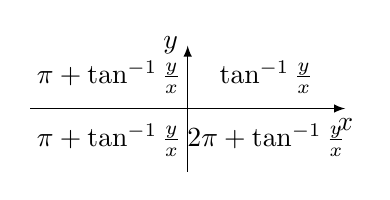
\begin{tikzpicture}
            % Achsen 
            \draw [-{latex}] (-2, 0) -- (2, 0) node [below] {$x$};
            \draw [-{latex}] (0, -0.8) -- (0, 0.8) node [left] {$y$};
            % Formeln
            \node at ( 1,  0.4) {$       \tan^{-1}\frac{y}{x}$};
            \node at ( 1, -0.4) {$2\pi + \tan^{-1}\frac{y}{x}$};
            \node at (-1, -0.4) {$ \pi + \tan^{-1}\frac{y}{x}$};
            \node at (-1,  0.4) {$ \pi + \tan^{-1}\frac{y}{x}$};
        \end{tikzpicture}
    \end{center}
\end{minipage}
\medskip

\myul{\textbf{Sphärisch $\rightarrow$ Zylindrisch:}}\\
\myul{\textbf{Kartesisch $\rightarrow$ Sphärisch:}}\\
Keine weiteren Berücksichtigungen nötig, die Berechnung erfolgt nach der Formel oben.
\medskip

\myul{\textbf{Zylindrisch $\rightarrow$ Sphärisch:}}\\
\begin{minipage}{0.49\linewidth}
    Auch hier macht der $\tan^{-1}$ Probleme, da er Werte von $-\frac{\pi}{2}$ bis $\frac{\pi}{2}$ liefert, für $\theta$ jedoch $\theta \in [0, \pi]$ gelten soll.
    Je nach dem, ob $P$ sich oberhalb oder unterhalb der $xy$-Ebene befindet, wird $\theta$ wie rechts berechnet.
\end{minipage}
\hfill
\begin{minipage}{0.49\linewidth}
    \begin{center}
        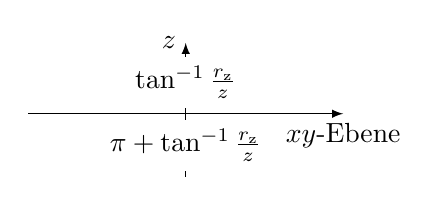
\begin{tikzpicture}
            % Achsen 
            \draw [-{latex}] (-2,  0)   -- (2, 0) node [below] {$xy$-Ebene};
            \draw [-{latex}] ( 0, -0.8) -- (0,.9) node [left]  {$z$};
            % Formeln
            \node [fill=white] at (0,  0.4) {$\tan^{-1}\frac{r_{\rm z}}{z}$};
            \node [fill=white] at (0, -0.4) {$\pi + \tan^{-1}\frac{r_{\rm z}}{z}$};
        \end{tikzpicture}
    \end{center}
\end{minipage}


        % DONE: Koordinatensysteme (Kartesisch, Polar, Kugel (Geografisch & Math.))

        \columnbreak
\section{Integration}
\subsection{Allgemeines}
Unter bi- oder multivariater Integration versteht man Integrale, welche sich über zwei oder mehr unabhängige Variablen erstrecken.
Sie haben die Form:
\[
    \int\limits_{\Omega} f(\omega) \diff \omega = \iint \cdots \int f(x_1, x_2, \ldots, x_n) \diff x_1 \diff x_2 \cdots \diff x_n
    \quad |\; \Omega \in \rreal^n
\]

\subsection{Normalbereiche}
Unter einem Normalbereich versteht man einen Bereich, welcher in allen Dimensionen so begrenzt ist, 
dass eine Funktion $f(x_1, x_2, \ldots, x_n)$ für jeden Eingangsvektor jeweils nur einen Funktionswert zurückgibt.


\example{Normalbereich in 2D}
\begin{center}
    \includegraphics[width=0.8\columnwidth]{images/Normalbereiche_2D.pdf}
\end{center}
% TODO: add caption


\subsection{Satz von Fubini (Satz von Tonelli)}
Der Satz von Fubini besagt, dass die Reihenfolge der Integrationen vertauscht werden kann, sofern die Funktion integrierbar ist.

\[
    \iint\limits_{y_1 x_1}^{\; y_2 x_2} f(x,y)\diff x \diff y = \iint\limits_{x_1 y_1}^{\; x_2 y_2} f(x,y)\diff y \diff x%\iint f(x, y) \diff x \diff y = \int \left\lgroup \int f(x, y) \diff x \right\rgroup \diff y = \int \left\lgroup \int f(x, y) \diff y \right\rgroup \diff x
\]

\subsection{Jacobi Matrix und Determinante}
Die Jacobi-Matrix besteht aus den partiellen Ableitungen eines Vektorfelds nach den Parametern.
\[
    \mathbf{J}_{\vec{f}} = \begin{pmatrix}
        \frac{\partial}{\partial x_1} f_1 & \frac{\partial}{\partial x_2} f_1 & \cdots & \frac{\partial}{\partial x_n} f_1\\
        \frac{\partial}{\partial x_1} f_2 & \frac{\partial}{\partial x_2} f_2 & \cdots & \frac{\partial}{\partial x_n} f_2\\
        \vdots & \vdots & \ddots & \vdots\\
        \frac{\partial}{\partial x_1} f_m & \frac{\partial}{\partial x_2} f_m & \cdots & \frac{\partial}{\partial x_n} f_m
    \end{pmatrix}
\]
Anhand der Jacobi-Matrix kann die Längen- und Flächenänderung bei einer Transformation berechnet werden.

\subsubsection{Transformation}
Koordinatensysteme können mit der Jacobi-Matrix allgemein in andere Systeme transformiert werden.

$T:(u, v) \xrightarrow{\text{T}} (x(u,v), y(u,v))$

Eine Transformation könnte dann beispielsweise wie folgt aussehen:
\[
    \diff x\diff y=\det(\mathbf{J}_T(u,v))\diff u \diff v,
\]
dabei ist $\det(\mathbf{J}_T(u,v))$ der Skalierungsfaktor.

\subsubsection{Längenverzerrung}
Die Längenverzerrung in eine Richtung $x_k$ ist definiert als: $\abs{\frac{\partial \vec{f}}{\partial x_k}} = \abs{\text{k. Spalte von }\mathbf{J}}$ 


\subsubsection{Elementverzerrung (Flächen- / Volumenverzerrung)}
Die Elementverzerrung ist definiert als: $\diff V' = \abs{\det \mathbf{J}}\cdot\diff V$ %da $\diff x_1 \diff x_2 \ldots \diff x_d = \det \mathbf{J} \diff u_1 \diff u_2 \ldots \diff u_d$


\subsubsection{Längenelement}
Ein Längenelement lässt sich ebenfalls aus der Jacobi Matrix berechnen:
\[
    \diff \vec{x}^2 = \diff\vec{x}\cdot\diff\vec{x} = (\diff\vec{u})^{\tr} \cdot (\mathbf{J}^{\tr} \cdot \mathbf{J}) \cdot (\diff\vec{u})
\]


\subsection{Erster Metrischer Tensor} % TODO: Vereinheitlichung d. Variablen und Funktionen
Der 1. metrische Tensor (oder auch \textbf{erste Fundamentalmatrix}, \textbf{erste Fundamentalform}, \textbf{metrische Grundform})
beschreibt den Zusammenhang zwischen einer Kurve oder Fläche im Parameterraum zum Raum, in dem sie sich befindet (z.B. 2D-Fläche im 3D-Raum).
Er besteht aus den Skalarprodukten der partiellen Ableitungsvektoren nach den Parametern.
\[
    \boxed{g_{ij} = \frac{\partial \vec{S}}{\partial u_i} \dotp \frac{\partial \vec{S}}{\partial u_j} = \mathbf{J}^{\tr} \cdot \mathbf{J}}
\]
Folglich ergibt sich die Matrix: $\begin{pmatrix}
    E & F\\
    F & G
\end{pmatrix} = \begin{pmatrix}
    g_{11} & g_{12}\\
    g_{21} & g_{22}
\end{pmatrix}$

Die Einträge dieser Matrix werden benötigt, um Längen- oder Flächen(elemente) zu berechnen.
Anhand der Einträge kann auch ausgesagt werden, ob eine Längen, Flächen und/oder Winkelerhaltung vorliegt:

\begin{minipage}[t]{0.33\columnwidth}
    \centering
    \myul{\textbf{Längenerhaltung}}

    \medskip
    $g_{ij} = \bm{I} = \begin{pmatrix}
        1 & 0 \\
        0 & 1 
    \end{pmatrix}$
\end{minipage}
\begin{minipage}[t]{.33\columnwidth}
    \centering
    \myul{\textbf{Flächenerhaltung}}

    \medskip
    $\det (g_{ij}) = 1$
\end{minipage}\hfill
\begin{minipage}[t]{.33\columnwidth}
    \centering
    \myul{\textbf{Winkelerhaltung}}

    \medskip
    Diagnonale 1. Fundamentalform:
    
    $(g_{11} = g_{22}) \land (g_{12} = g_{21} = 0)$
\end{minipage}


% DONE: subsubsection Flächen-, Längen- & Winkelerhaltung (Siehe Moodle Woche 11)
\example{Längenberechnung}
Gegeben: Flächenkurve als $\vec{x}(t) = \begin{pmatrix}
    u(t)\\
    v(t)
\end{pmatrix}$

\medskip
Totales Differential bilden: 
\hfill\parbox{.5\columnwidth}{\centering $\displaystyle \diff s^2 = \dot{\vec{x}} = \vec{x}_u \cdot \dot{u} + \vec{x}_v \cdot \dot{v}$}

\medskip
Für Längenelement Pythagoras anwenden: 
\hfill\parbox{.48\columnwidth}{\centering $\displaystyle (\dot{\vec{x}})^2 = g_{11} \dot{u}^2 + 2 g_{12} \dot{u} \dot{v} + g_{22} \dot{v}^2$}

\medskip
Das einzelne Längenelement ist somit:
\hfill\parbox{.48\columnwidth}{\centering $\displaystyle \diff s = \sqrt{g_{11} \diff u^2 + 2 g_{12} \diff u \diff v + g_{22} \diff v^2}$}

\medskip
$\diff s$ integrieren, für Gesamtlänge: 
\hfill\parbox{.48\columnwidth}{\centering $\displaystyle s = \int\limits_{a}^{b} \sqrt{g_{11} \dot{u}^2 + 2 g_{12} \dot{u} \dot{v} + g_{22} \dot{v}^2} \diff t$}


\example{Flächenberechnung}
Es sei eine parametrisierte Fläche als Funktion $\vec{S}(u,v) = \begin{pmatrix}
    x(u,v)\\
    y(u,v)\\
    z(u,v)
\end{pmatrix}$ gegeben.
Das Flächenelement lässt sich aus einem Parallelogramm der beiden partiellen Ableitungsvektoren bilden, 
was dem Betrag des Kreuzproduktes bzw. der Determinante entspricht:
\[
    \diff S = \sqrt{\abs{\det\abs{g_{ij}}}}\diff u \diff v = \sqrt{g_{11}g_{22} - g_{12}^2} \diff u \diff v = \abs{\frac{\partial \vec{S}}{\partial u} \times \frac{\partial \vec{S}}{\partial v}} \diff u \diff v
\]
Daraus ergibt sich die Fläche über das Doppelintegral:
\[
    S = \iint\limits_{v_1\, u_1}^{v_2\, u_2} \sqrt{g_{11}g_{22} - g_{12}^2} \diff u \diff v
\]


% DONE: Längenintegrale (3D)
% TODO: Längenintegrale (2D)
\subsection{Längenintegrale}
\subsubsection{Längenelemente}\label{section:int_multivar:längenelemente}
$$
 \diff s^2 
    = \underbrace{\diff x^2 + \diff y^2 + \diff z^2}_{\text{Kartesisch}}
    = \underbrace{\diff r^2 + r^2 \diff \varphi^2 + \diff z^2}_{\text{Zylindrisch}}
    = \underbrace{\diff r^2 + r^2 \diff \theta^2 + r^2 \sin^2 \theta \diff \phi^2}_{\text{Sphärisch}}
$$
\subsubsection{Kurvenintegrale 1. Art: Länge einer Funktion}
Die Bestimmung der Länge einer Kurve kann in folgende Schritte unterteilt werden:
\begin{enumerate}
    \item \myul{\textbf{Funktion in die Parameterdarstellung überführen (sofern nicht gegeben):}}
    \item[] Dafür wird einer der Parameter (z.B. $x$ oder $\theta$) $=t$ gesetzt und die anderen Parameter ebenfalls als Funktion von $t$ ausgedrückt.
    \item \myul{\textbf{Integral aufstellen:}}
    \item[] Das Integral in der Form $ \iiint \diff s $ wird mit $\frac{\diff t}{\diff t}$ erweitert.
    \item \myul{\textbf{Das Integral lösen}}
\end{enumerate}

% \subsubsection{Beispiel}
\example{Längenintegral in kartesischen Koordinaten}
Es soll die Länge der Kurve $\vec{v}(t) = \begin{pmatrix}x(t)\\y(t)\\z(t)\end{pmatrix}$ auf dem Interval $[t_1, t_2]$ bestimmt werden.
Dazu werden die oben genannten Schritte abgearbeitet:
\begin{enumerate}
    \item \textbf{Funktion in die Parameterdarstellung überführen}
    \item[] Hier nicht nötig. % evtl. TODO: Beispiel wählen, bei dem das nötig ist.
    \item \textbf{Integral aufstellen} 
    \item[] $ \iiint \diff s = \iiint \sqrt{\diff x^2 + \diff y^2 + \diff z^2} = \int_{t_1}^{t_2} \sqrt{\left(\frac{\diff x}{\diff t}\right)^2 + \left(\frac{\diff y}{\diff t}\right)^2 + \left(\frac{\diff z}{\diff t}\right)^2} \diff t$
    \item Integral lösen
    \item[] $\frac{\diff x}{\diff t}$, $\frac{\diff y}{\diff t}$ und $\frac{\diff z}{\diff t}$ ausrechnen, einsetzen, integrieren.
\end{enumerate}

\subsubsection{Kurvenintegral 2. Art}
Beim Kurvenintegral 2. Art wird nicht die tatsächliche Länge einer Funktion, sondern die Länge deren Projektion auf eine Achse bestimmt.
Dazu wird stat über alle Koordinatenrichtungen nur über eine der Koordinaten integriert.

Es folgen einige Paare von Kurvenintegralen 2. Art entlang einer Kontur $K$ für Funktionen in expliziter Form und in Parameterdarstellung.

\myul{2D, Projektion auf x:}
\[
    \int\limits_{K}f(x)dx = \int_{t_0}^{T}\vec{f}(x(t), y(t)) \cdot x'(t) \cdot dt
\]

\myul{3D, Projektion auf x:}
\[
    \int\limits_{K}f(x, y)dx = \int_{t_0}^{T}\vec{f}(x(t), y(t), z(t)) \cdot x'(t) \cdot dt
\]


% DONE: Flächenintegrale (2D, 3D)
\subsection{(Ober-)Flächenintegrale}
\subsubsection{Flächenelemente}
Das Bestimmen der Flächenelemente ist in drei Dimensionen nicht wie bei den Längen- und Volumenelementen pauschal möglich.
Dies, da jeweils nur über zwei der drei Koordinaten integriert werden muss.
Ein einfaches Verfahren für das Berechnen von Flächeninhalten schafft jedoch abhilfe.

\subsubsection{Flächeninhalt einer Oberfläche}
Für das Berechnen der Oberflächen von Funktionen des Typs $f(a, b)$ in 3D kann die Formel
$$ S = \int\limits_{B} \int\limits_{A} \sqrt{(f_{a})^2 + (f_{b})^2 + 1} \diff a \diff b $$
verwendet werden. Dabei repräsentieren $a$ und $b$ die beiden Koordinatenrichtungen, in denen sich die Fläche erstreckt.
$f_a$ und $f_b$ sind die partiellen Ableitungen der Funktion $f(a, b)$ nach $a$ bzw. $b$.
\medskip

\myul{\bf{Beispiele zur Veranschaulichung:}}\\
Es soll die Oberfläche der Funktion $ f(x, y) $ im Bereich $ x \in [x_1, x_2], y \in [y_1, y_2] $ bestimmt werden.
Das entsprechende integral lautet:
$$ S = \int_{y_1}^{y_2} \int_{x_1}^{x_2} \sqrt{(f_{x})^2 + (f_{y})^2 + 1} \diff x \diff y $$

% Wäre die Funktion $f$ stat in kartesischen in polaren oder sphärischen Koordinaten formuliert, ändern sich lediglich die Namen der Variablen. 
% Folglich ist das zu einer in sphärischen Koordinaten definierten Fkt. $f(\theta, \phi)$ gehörende Integral
% $$ S = \int_{\phi_1}^{\phi_2} \int_{\theta_1}^{\theta_2} \sqrt{(f_{\theta})^2 + (f_{\phi})^2 + 1} \diff \theta \diff \phi $$
% sehr leicht aufzustellen.


\subsubsection{Allgemeine Wendelfläche}
Die allgemeine Wendelfläche rotiert und verschiebt eine parametrisierte 3D Kurve $\vec{r}(t) = (x(t), y(t), z(t))\tr$ im Raum.

Parametrisierung bei vertikaler Rotationsachse und vertikaler Verschiebungsrichtung ($z$-Achse):
\[
    \vec{S}(t, \varphi) = \begin{pmatrix}
        \begin{pmatrix}
            \cos(\varphi) & -\sin(\varphi)\\
            \sin(\varphi) & \cos(\varphi)
        \end{pmatrix}
        \cdot \begin{pmatrix}
            x(t)\\
            y(t)
        \end{pmatrix}\\
        z(t) + c \cdot \varphi
    \end{pmatrix}
    \quad (t_1 \leq t \leq t_2, \land \varphi \in \rreal\;, c \equiv const.)
\]

Bei $c = 1$ \textrightarrow\ Voller Meter bei einer Kurve % TODO: Check this



% TODO: Volumenintegrale (3D)
\subsection{Volumenintegrale}
\subsubsection{Volumenelemente}
$$ 
 \diff V 
    = \underbrace{\diff x \diff y \diff z}_{\text{Kartesisch}}
    = \underbrace{r \diff r \diff \varphi \diff z}_{\text{Zylindrisch}}
    = \underbrace{r^2 \sin \theta \diff \theta \diff \phi \diff r}_{\text{Sphärisch}}
$$


% TODO: Andwendungsformeln
% \subsection{Anwendungsformeln}
% TODO: Anwendungsformeln 2D (Doppelintegrale)
% custom big strut for vertical spacing in tables
\subsection{Anwendungsformeln 2D (Doppelintegrale)}
\resizebox{\linewidth}{!}{
    \begin{tabular}{|l|l|l|}
        \hline
        \bf{Allgemein} & \bf{Kartesische Koordinaten} & \bf{Polarkoordinaten} \\
        \hline

        \multicolumn{3}{|l|}{\bf{Flächeninhalt einer ebenen Figur $F$}} \\\hline
        \bigstrut[tb]$\mathstrut A = \iint\limits_{F} \diff F $ & 
        $ = \int\limits_{X}\int\limits_{Y} \diff y \diff x $ &
        $ = \int\limits_{\Phi}\int\limits_{R} r \diff r \diff \varphi $ \\\hline

        \multicolumn{3}{|l|}{\bf{Oberfläche einer Ebene in drei Dimensionen}} \\\hline
        % TODO: Evtl. umschreiben, dass man es besser versteht...
        \bigstrut[tb]$ S = \iint\limits_{A} \frac{1}{\cos \gamma} \diff A $ & 
        $ = \int\limits_{X}\int\limits_{Y} \sqrt{1 + \left(\frac{\partial z}{\partial x}\right)^2 + \left(\frac{\partial z}{\partial y}\right)^2} \diff y \diff x $ &
        $ = \int\limits_{\Phi}\int\limits_{R} \sqrt{r^2 + r^2\left(\frac{\partial z}{\partial r}\right)^2 + \left(\frac{\partial z}{\partial \varphi}\right)^2} \diff r \diff \varphi $ \\\hline
        
        \multicolumn{3}{|l|}{\bf{Volumen eines Zylinders}} \\\hline
        \bigstrut[tb]$ V = \iint\limits_{A} z \diff A $ & 
        $ = \int\limits_{X}\int\limits_{Y} z \diff y \diff x $ &
        $ = \int\limits_{\Phi}\int\limits_{R} z r \diff r \diff \varphi $ \\\hline

        \multicolumn{3}{|l|}{\bf{Trägheitsmoment einer ebenen Figur $F$, bezogen auf die x-Achse}} \\\hline
        \bigstrut[tb]$ I_x = \iint\limits_{F} y^2 \diff F $ & 
        $ = \int\limits_{X}\int\limits_{Y} (y^2) \diff y \diff x $ &
        $ = \int\limits_{\Phi}\int\limits_{R} (r^2 \sin^2\varphi) r \diff r \diff \varphi $ \\\hline

        \multicolumn{3}{|l|}{\bf{Trägheitsmoment einer ebenen Figur $F$, bezogen auf den Pol $(0, 0)$}} \\\hline
        \bigstrut[tb]$ I_x = \iint\limits_{F} r^2 \diff F $ & 
        $ = \int\limits_{X}\int\limits_{Y} (x^2 + y^2) \diff y \diff x $ &
        $ = \int\limits_{\Phi}\int\limits_{R} (r^2) r \diff r \diff \varphi $ \\\hline

        \multicolumn{3}{|l|}{\bf{Masse einer ebenen Figur $F$ mit Dichtefunktion $\varrho$}} \\\hline
        \bigstrut[tb]$ m = \iint\limits_{F} \varrho \diff F $ & 
        $ = \int\limits_{X}\int\limits_{Y} \varrho (x, y) \diff y \diff x $ &
        $ = \int\limits_{\Phi}\int\limits_{R} \varrho (r, \varphi) r \diff r \diff \varphi $ \\\hline

        \multicolumn{3}{|l|}{\bf{Koordinaten des Schwerpunkts $S$ einer homogenen, ebenen Figur $F$}} \\\hline
        \bigstrut[tb]$ x_{S} = \frac{\strut \iint\limits_{F} x \diff F}{A} $ & 
        $ = \frac{\int\limits_{X}\int\limits_{Y} x \diff y \diff x}{\int\limits_{X}\int\limits_{Y} \diff y \diff x} $ &
        $ = \frac{\int\limits_{\Phi}\int\limits_{R} r^2 \cos \varphi \diff r \diff \varphi}{\int\limits_{\Phi}\int\limits_{R} r \diff r \diff \varphi} $ \\
        \bigstrut[tb]$ y_{S} = \frac{\iint\limits_{F} y \diff F}{A} $ & 
        $ = \frac{\int\limits_{X}\int\limits_{Y} y \diff y \diff x}{\int\limits_{X}\int\limits_{Y} \diff y \diff x} $ &
        $ = \frac{\int\limits_{\Phi}\int\limits_{R} r^2 \sin \varphi \diff r \diff \varphi}{\int\limits_{\Phi}\int\limits_{R} r \diff r \diff \varphi} $ \\\hline
    \end{tabular}
}

\smallskip
Hinweis: Damit die Flächenelemente leichter erkennbar und die Formeln entsprechend besser nachvollziebar sind, wurden sie teilweise nicht vollständig vereinfacht.


% TODO: Anwendungsformeln 3D (Dreifachintegrale)
\subsection{Anwendungsformeln 3D (Dreifachintegrale)}
\resizebox{\linewidth}{!}{
    \begin{tabular}{|l|l|l|l|}  
        \hline
        \bf{Allgemein} & \bf{Kartesische Koordinaten} & \bf{Zylinderkoordinaten} & \bf{Kugelkoordinaten} \\
        \hline
        \multicolumn{4}{|l|}{\bf{Oberfläche eines Körpers $K$ (Senkrecht zu $\hat{a}_r$)}} \\
        \hline
        \bigstrut[tb]$ S = \iint\limits_{K} \diff S $ & 
        \textsl{Siehe metrischer Tensor}&%$ = \iint \diff x \diff y \diff z $ &
        $ = \iint r \diff \varphi \diff z $ &
        $ = \iint r^2 \sin \theta \diff \theta \diff \phi $ \\
        \hline

        \multicolumn{4}{|l|}{\bf{Volumen eines Körpers $K$}} \\
        \hline
        \bigstrut[tb]$ V = \iiint\limits_{K} \diff V $ & 
        $ = \iiint \diff x \diff y \diff z $ &
        $ = \iiint r \diff r \diff \varphi \diff z $ &
        $ = \iiint r^2 \sin \theta \diff \theta \diff \phi \diff r $ \\
        \hline

        \multicolumn{4}{|l|}{\bf{Trägheitsmoment eines Körpers $K$, bezogen auf die Z-Achse}} \\
        \hline
        \bigstrut[tb]$ I_z = \iiint\limits_{K} r^2 \diff V $ & 
        $ = \iiint (x^2 + y^2) \diff x \diff y \diff z $ &
        $ = \iiint (r^2) r \diff r \diff \varphi \diff z $ &
        $ = \iiint (r^2 \sin^2 \theta) r^2 sin \theta \diff \theta \diff \phi \diff r $ \\
        \hline

        \multicolumn{4}{|l|}{\bf{Masse eines Körpers $K$ mit der Dichtefunktion $\varrho$}} \\
        \hline
        \bigstrut[tb]$ M = \iiint\limits_{K} \varrho \diff V $ & 
        $ = \iiint \varrho (x, y, z) \diff x \diff y \diff z $ &
        $ = \iiint \varrho (r, \varphi, z) r \diff r \diff \varphi \diff z $ &
        $ = \iiint \varrho (r, \theta, \phi) r^2 sin \theta \diff \theta \diff \phi \diff r $ \\
        \hline

        \multicolumn{4}{|l|}{\bf{Koordinaten des Schwerpunktes $S$ eines homogenen Körpers $K$}} \\
        \hline
        $ x_{S} = \frac{\strut \iiint\limits_{K} x \diff V}{V} $ & 
        $ = \frac{\iiint (x) \diff x \diff y \diff z}{V} $ &
        $ = \frac{\iiint (r \cos \varphi) r \diff r \diff \varphi \diff z}{V} $ &
        $ = \frac{\iiint (r \sin \theta \cos \phi) r^2 sin \theta \diff \theta \diff \phi \diff r}{V} $ \\

        \bigstrut[tb]$ y_{S} = \frac{\iiint\limits_{K} y \diff V}{V} $ & 
        $ = \frac{\iiint (y) \diff x \diff y \diff z}{V} $ &
        $ = \frac{\iiint (r \sin \varphi) r \diff r \diff \varphi \diff z}{V} $ &
        $ = \frac{\iiint (r \sin \theta \sin \phi) r^2 sin \theta \diff \theta \diff \phi \diff r}{V} $ \\

        \bigstrut[tb]$ z_{S} = \frac{\iiint\limits_{K} z \diff V}{V} $ & 
        $ = \frac{\iiint (z) \diff x \diff y \diff z}{V} $ &
        $ = \frac{\iiint (z) r \diff r \diff \varphi \diff z}{V} $ &
        $ = \frac{\iiint (r \cos \theta) r^2 sin \theta \diff \theta \diff \phi \diff r}{V} $ \\
        \hline
    \end{tabular}
}

\smallskip
Hinweis: Damit die Volumenelemente leichter erkennbar und die Formeln entsprechend besser nachvollziebar sind, wurden sie teilweise nicht vollständig vereinfacht.

% TODO: What is with this huge ass comment?!
% \subsection{Umrechnungen}
% \subsubsection{Kartesische Koordinaten $\leftrightarrow$ Polarkoordinaten}

% \subsection{Anwendungsformeln}
% \resizebox{\linewidth}{!}{
%     \begin{tabular}{|l|l|l|}
%         \hline
%         \bf{Allgemein} & \bf{Kartesische Koordinaten} & \bf{Polarkoordinaten} \\
%         \hline

%         \multicolumn{3}{|l|}{\bf{Flächeninhalt einer ebenen Figur $F$}} \\\hline
%         $ A = \iint\limits_{F} \diff a $ & 
%         $ = \int\limits_{X}\int\limits_{Y} \diff y \diff x $ &
%         $ = \int\limits_{\Phi}\int\limits_{R} r \diff r \diff \varphi $ \\\hline

%         \multicolumn{3}{|l|}{\bf{Oberfläche einer Ebene in drei Dimensionen}} \\\hline
%         % TODO: Evtl. umschreiben, dass man es besser versteht...
%         $ S = \iint\limits_{A} \frac{1}{\cos \gamma} \diff a $ & 
%         $ = \int\limits_{X}\int\limits_{Y} \sqrt{1 + \left(\frac{\partial z}{\partial x}\right)^2 + \left(\frac{\partial z}{\partial y}\right)^2} \diff y \diff x $ &
%         $ = \int\limits_{\Phi}\int\limits_{R} \sqrt{r^2 + r^2\left(\frac{\partial z}{\partial r}\right)^2 + \left(\frac{\partial z}{\partial \varphi}\right)^2} \diff r \diff \varphi $ \\\hline
        
%         \multicolumn{3}{|l|}{\bf{Volumen eines Zylinders}} \\\hline
%         $ V = \iint\limits_{A} z \diff a $ & 
%         $ = \int\limits_{X}\int\limits_{Y} z \diff y \diff x $ &
%         $ = \int\limits_{\Phi}\int\limits_{R} z r \diff r \diff \varphi $ \\\hline

%         \multicolumn{3}{|l|}{\bf{Trägheitsmoment einer ebenen Figur $F$, bezogen auf die x-Achse}} \\\hline
%         $ I_x = \iint\limits_{F} y^2 \diff a $ & 
%         $ = \int\limits_{X}\int\limits_{Y} (y^2) \diff y \diff x $ &
%         $ = \int\limits_{\Phi}\int\limits_{R} (r^2 \sin^2\varphi) r \diff r \diff \varphi $ \\\hline

%         \multicolumn{3}{|l|}{\bf{Trägheitsmoment einer ebenen Figur $F$, bezogen auf den Pol $(0, 0)$}} \\\hline
%         $ I_x = \iint\limits_{F} r^2 \diff a $ & 
%         $ = \int\limits_{X}\int\limits_{Y} (x^2 + y^2) \diff y \diff x $ &
%         $ = \int\limits_{\Phi}\int\limits_{R} (r^2) r \diff r \diff \varphi $ \\\hline

%         \multicolumn{3}{|l|}{\bf{Masse einer ebenen Figur $F$ mit Dichtefunktion $\varrho$}} \\\hline
%         $ m = \iint\limits_{F} \varrho \diff a $ & 
%         $ = \int\limits_{X}\int\limits_{Y} \varrho (x, y) \diff y \diff x $ &
%         $ = \int\limits_{\Phi}\int\limits_{R} \varrho (r, \varphi) r \diff r \diff \varphi $ \\\hline

%         \multicolumn{3}{|l|}{\bf{Koordinaten des Schwerpunkts $S$ einer homogenen, ebenen Figur $F$}} \\\hline
%         $ x_{S} = \frac{\iint\limits_{F} x \diff a}{A} $ & 
%         $ = \frac{\int\limits_{X}\int\limits_{Y} x \diff y \diff x}{\int\limits_{X}\int\limits_{Y} \diff y \diff x} $ &
%         $ = \frac{\int\limits_{\Phi}\int\limits_{R} r^2 \cos \varphi \diff r \diff \varphi}{\int\limits_{\Phi}\int\limits_{R} r \diff r \diff \varphi} $ \\
%         $ y_{S} = \frac{\iint\limits_{F} y \diff a}{A} $ & 
%         $ = \frac{\int\limits_{X}\int\limits_{Y} y \diff y \diff x}{\int\limits_{X}\int\limits_{Y} \diff y \diff x} $ &
%         $ = \frac{\int\limits_{\Phi}\int\limits_{R} r^2 \sin \varphi \diff r \diff \varphi}{\int\limits_{\Phi}\int\limits_{R} r \diff r \diff \varphi} $ \\\hline
%     \end{tabular}
% }

% \resizebox{\linewidth}{!}{
%     \begin{tabular}{|l|l|l|l|}  
%         \hline
%         \bf{Allgemein} & \bf{Kartesische Koordinaten} & \bf{Zylinderkoordinaten} & \bf{Kugelkoordinaten} \\
%         \hline
%         \multicolumn{4}{|l|}{\bf{Volumen eines Körpers $K$}} \\
%         \hline
%         $ V = \iiint\limits_{K} \diff V $ & 
%         $ = \iiint \diff x \diff y \diff z $ &
%         $ = \iiint r \diff r \diff \phi \diff z $ &
%         $ = \iiint r^2 \sin \theta \diff \theta \diff \phi \diff r $ \\
%         \hline

%         \multicolumn{4}{|l|}{\bf{Trägheitsmoment eines Körpers $K$, bezogen auf die Z-Achse}} \\
%         \hline
%         $ I_z = \iiint\limits_{K} r^2 \diff V $ & 
%         $ = \iiint (x^2 + y^2) \diff x \diff y \diff z $ &
%         $ = \iiint (r^2) r \diff r \diff \phi \diff z $ &
%         $ = \iiint (r^2 \sin^2 \theta) r^2 sin \theta \diff \theta \diff \phi \diff r $ \\
%         \hline

%         \multicolumn{4}{|l|}{\bf{Masse eines Körpers $K$ mit der Dichtefunktion $\varrho$}} \\
%         \hline
%         $ M = \iiint\limits_{K} \varrho \diff V $ & 
%         $ = \iiint \varrho (x, y, z) \diff x \diff y \diff z $ &
%         $ = \iiint \varrho (r, \phi, z) r \diff r \diff \phi \diff z $ &
%         $ = \iiint \varrho (r, \theta, \phi) r^2 sin \theta \diff \theta \diff \phi \diff r $ \\
%         \hline

%         \multicolumn{4}{|l|}{\bf{Koordinaten des Schwerpunktes $S$ eines homogenen Körpers $K$}} \\
%         \hline
%         $ x_{S} = \frac{\iiint\limits_{K} x \diff V}{V} $ & 
%         $ = \frac{\iiint (x) \diff x \diff y \diff z}{V} $ &
%         $ = \frac{\iiint (r \cos \phi) r \diff r \diff \phi \diff z}{V} $ &
%         $ = \frac{\iiint (r \sin \theta \cos \phi) r^2 sin \theta \diff \theta \diff \phi \diff r}{V} $ \\

%         $ y_{S} = \frac{\iiint\limits_{K} y \diff V}{V} $ & 
%         $ = \frac{\iiint (y) \diff x \diff y \diff z}{V} $ &
%         $ = \frac{\iiint (r \sin \phi) r \diff r \diff \phi \diff z}{V} $ &
%         $ = \frac{\iiint (r \sin \theta \sin \phi) r^2 sin \theta \diff \theta \diff \phi \diff r}{V} $ \\

%         $ z_{S} = \frac{\iiint\limits_{K} z \diff V}{V} $ & 
%         $ = \frac{\iiint (z) \diff x \diff y \diff z}{V} $ &
%         $ = \frac{\iiint (z) r \diff r \diff \phi \diff z}{V} $ &
%         $ = \frac{\iiint (r \cos \theta) r^2 sin \theta \diff \theta \diff \phi \diff r}{V} $ \\
%         \hline
%     \end{tabular}
% }



% \section{Koordinatensysteme}
% \subsection{2D Koordinatensysteme}
% Neben den Kartesischen Koordinatensystemen kommen in zweidimensionalen Räumen auch Polare Koordinatensysteme zum Einsatz.
% Die beiden Systeme können mit Hilfe der Trigonometrie in einander überführt werden.

% \subsubsection{Umrechnung Kartesisch $\leftrightarrow$ Polar}
% \begin{minipage}{0.29\linewidth}
%     \myul{Polar zu Kartesisch}
%     \[
%     \begin{pmatrix}
%         x \\
%         y
%     \end{pmatrix}
%     =
%     \begin{pmatrix}
%         r \cdot \cos{\varphi}\\
%         r \cdot \sin{\varphi}
%     \end{pmatrix}
%     \]
% \end{minipage}
% \hfill
% \begin{minipage}{0.29\linewidth}
%     \myul{Kartesisch zu Polar}
%     \[
%     \begin{pmatrix}
%         r \\
%         \varphi
%     \end{pmatrix}
%     =
%     \begin{pmatrix}
%         \sqrt{x^2+y^2}\\
%         \tan^{-1}{\frac{y}{x}}
%     \end{pmatrix}
%     \]
% \end{minipage}
% \hfill
% \begin{minipage}{0.29\linewidth}
%     \begin{center}
%         \begin{tikzpicture} [scale = 1.5]
%             % Kartesische Achsen
%             \draw[-{latex}] (0, 0) -- (1, 0) node [below] {$x$} ;
%             \draw[-{latex}] (0, 0) -- (0, 1) node [left]  {$y$} ;

%             % Punkt p
%             \fill (0.5, 0.8) circle (1pt) node [anchor=south west] {$\vec{p}$};

%             % Länge r
%             \draw (0, 0) -- (0.5, 0.8) node [midway, above left] {$r$};
%             % Winkel phi
%             \draw [-{latex}] (0.5, 0) arc (0:58:0.5) node [midway, right] {$\varphi$};
%         \end{tikzpicture}
%     \end{center}
% \end{minipage}

% Dabei ist zu beachten, dass $\tan^{-1}$ nur werte von $-\frac{\pi}{2}$ bis $\frac{\pi}{2}$ liefert, für $\varphi$ jedoch $\varphi \in [0, \pi]$ gelten soll. 
% $\varphi$ wird also, je nach dem in welchem Quadranten sich $\vec{p}$ befindet, nach folgendem Schema berechnet:
% \begin{center}
%     \begin{tikzpicture}
%         % Achsen 
%         \draw [-{latex}] (-2, 0) -- (2, 0) node [below] {$x$};
%         \draw [-{latex}] (0, -0.8) -- (0, 0.8) node [left] {$y$};
%         % Formeln
%         \node at ( 1,  0.4) {$       \tan^{-1}\frac{y}{x}$};
%         \node at ( 1, -0.4) {$2\pi + \tan^{-1}\frac{y}{x}$};
%         \node at (-1, -0.4) {$\pi  + \tan^{-1}\frac{y}{x}$};
%         \node at (-1,  0.4) {$\pi  + \tan^{-1}\frac{y}{x}$};
%     \end{tikzpicture}
% \end{center}

% Um eine ganzes Integral vom einen Koordinatensystem ins andere zu überführen, muss zum einen die Funktion $ f(x, y) $ zu $ f(r, \varphi) $ (oder umgekehrt) umgeschrieben, sowie die differentiale angepasst werden.
% Hier dafür einige gängige Elemente:

% \begin{tabular}{l c c}
%                          & \bf{Kartesisch}                   & \bf{Polar}                                                       \\
%     \bf{x-Achsenelement} & $\diff x$                         & $\diff x = \cos \varphi \diff r - r \sin \varphi \diff \varphi$  \\
%     \bf{y-Achsenelement} & $\diff y$                         & $\diff x = \sin \varphi \diff r + r \cos \varphi \diff \varphi$  \\
%     \bf{Linienelement  } & $\diff s^2 = \diff x^2 \diff y^2$ & $\diff s^2 = \diff r^2 + r^2 \diff \varphi^2$                    \\
%     \bf{Flächenelement } & $\diff A = \diff x \diff y$       & $\diff A = r \diff r \diff \varphi$                              \\
% \end{tabular}

% % \subsection{2D Transformation Polar zu Kartesisch}
% % TODO: Das isch ja ds gliiche wie obe beschribe, oder?
% %       Wänn da no meh ane sött wüsstich nöd was... -Flurin
% % T $=$ Transformation
% % \[
% %     \text{Polar } (r,\varphi) \xrightarrow{T} (x,y) \text{ Kartesisch}
% % \]

% % \[
% % \begin{pmatrix}
% %     x=r\cdot\cos(\varphi) \text{ } \cor{\mathbb{R}} \\
% %     y=r\cdot\sin(\varphi) \text{ } \cor{\mathbb{R}} 
% % \end{pmatrix}
% % \text{2D}
% % \]

% % Die Funktionen für $x$ und $y$ sind skalare Funktion.

% %     \begin{ctabular}{ll}
% %         $x=x(r;\varphi)$ & $ y=y(r;\varphi)$
% %     \end{ctabular}


% \subsection{3D Koordinatensysteme}
% \resizebox{\linewidth}{!}{
%     \begin{tabular}{c c c}
%         \myul{\textbf{Kartesisch}} & \myul{\textbf{Zylindrisch}} & \myul{\textbf{Sphärisch}} \\
        
%         \tdplotsetmaincoords{70}{110}
%         \begin{tikzpicture}[baseline=(current bounding box.north), tdplot_main_coords, scale=2]
%             % Koordinatensystem
%             \draw [-{latex}] (0, 0, 0) -- (1, 0, 0) node [below left] {$x$};
%             \draw [-{latex}] (0, 0, 0) -- (0, 1, 0) node [right]      {$y$};
%             \draw [-{latex}] (0, 0, 0) -- (0, 0, 1) node [right]      {$z$};
%             % Punkt bei (0.75,0.75,0.75)
%             \fill (0.75, 0.75, 0.75) circle (1pt) node [above right] {$P(x, y, z)$};
%             % Koordinatenkomponenten
%             \draw [dashed] (0, 0.75, 0)    -- (0.75, 0.75, 0)    node [midway, below right] {$x$};
%             \draw [dashed] (0.75, 0, 0)    -- (0.75, 0.75, 0)    node [midway, below left]  {$y$};
%             \draw [dashed] (0.75, 0.75, 0) -- (0.75, 0.75, 0.75) node [midway, right]       {$z$};
%         \end{tikzpicture} &

%         \tdplotsetmaincoords{70}{110}
%         \begin{tikzpicture}[baseline=(current bounding box.north), tdplot_main_coords, scale=2]
%             % Koordinatensystem
%             \draw [-{latex}] (0, 0, 0) -- (1, 0, 0) node [below left] {$x$};
%             \draw [-{latex}] (0, 0, 0) -- (0, 1, 0) node [right]      {$y$};
%             \draw [-{latex}] (0, 0, 0) -- (0, 0, 1) node [right]      {$z$};
%             % Punkt bei (0.75,0.75,0.75)
%             \fill (0.75, 0.75, 0.75) circle (1pt) node [above right] {$P(r_{\rm z}, \varphi, z)$};
%             % Koordinatenkomponenten
%             \draw [dashed] (0,0,0)         --  (0.75, 0.75, 0)    node [midway, above right, inner sep=0pt] {$r_{\rm z}$};
%             \draw [-{latex}]     (0.5,0,0)       arc (0:45:0.5)         node [midway, below]       {$\varphi$};
%             \draw [dashed] (0.75, 0.75, 0) --  (0.75, 0.75, 0.75) node [midway, right]       {$z$};
%         \end{tikzpicture} &

%         \tdplotsetmaincoords{70}{110}
%         \begin{tikzpicture}[baseline=(current bounding box.north), tdplot_main_coords, scale=2]
%             % Koordinatensystem
%             \draw [-{latex}] (0, 0, 0) -- (1, 0, 0) node [below left] {$x$};
%             \draw [-{latex}] (0, 0, 0) -- (0, 1, 0) node [right]      {$y$};
%             \draw [-{latex}] (0, 0, 0) -- (0, 0, 1) node [right]      {$z$};
%             % Punkt bei (0.75,0.75,0.75)
%             \fill (0.75, 0.75, 0.75) circle (1pt) node [above right] {$P(r_{\rm s}, \theta, \phi)$};
%             % Koordinatenkomponenten
%             \draw [dotted] (0,0,0) -- (0.75, 0.75, 0) -- (0.75, 0.75, 0.75);
%             \draw [-{latex}]     (0.5,0,0) arc (0:45:0.5)         node [midway, below]       {$\phi$};
%             \draw [dashed] (0, 0, 0) --  (0.75, 0.75, 0.75) node [midway, below right] {$r_{\rm s}$};
%             \tdplotsetthetaplanecoords {90}
%             \tdplotdrawarc [tdplot_rotated_coords, -{latex}] {(0, 0, 0)} {0.5} {0} {45} {anchor=south} {$\theta$}
%         \end{tikzpicture} \\

%         $ 
%         \begin{pmatrix}
%             x \\ y \\ z
%         \end{pmatrix} 
%         =
%         \begin{pmatrix}
%             r \cos \varphi \\ r \sin \varphi \\ z
%         \end{pmatrix}
%         =
%         \begin{pmatrix}
%             r \sin \theta \cos \phi \\ r \sin \theta \sin \phi \\ r \cos \theta
%         \end{pmatrix}
%         $ &
%         $ 
%         \begin{pmatrix}
%             r_{\rm z} \\ \varphi \\ z
%         \end{pmatrix} 
%         =
%         \begin{pmatrix}
%             \sqrt{x^2 + y^2} \\ \tan^{-1}\frac{y}{x} \\ z
%         \end{pmatrix}
%         =
%         \begin{pmatrix}
%             r_{\rm s} \sin \theta \\ \phi \\ r_{\rm s} \cos \theta
%         \end{pmatrix}
%         $ &
%         $ 
%         \begin{pmatrix}
%             r_{\rm s} \\ \theta \\ \phi
%         \end{pmatrix} 
%         =
%         \begin{pmatrix}
%             \sqrt{x^2+y^2+z^2} \\ \cos^{-1} \frac{z}{\sqrt{x^2+y^2+z^2}} \\ \sgn(y) \cos^{-1} \frac{x}{\sqrt{x^2+y^2}}
%         \end{pmatrix}
%         =
%         \begin{pmatrix}
%             \sqrt{r_{\rm z}^2+z^2} \\ \tan^{-1}\frac{r_{\rm z}}{z} \\ \varphi
%         \end{pmatrix}
%         $ \\
%     \end{tabular}
% }
% \smallskip
% \subsubsection{Umrechnen zwischen Koordinatensystemen}
% Beim Umrechnen zwischen den Koordinatensystemen gelten im Grunde genommen die obigen Formeln. 
% Dabei muss jedoch in einigen Fällen auf die Wertebereiche von den trigonometrischen Funktionen rücksicht genommen werden.

% \myul{\textbf{Zylindrisch $\rightarrow$ Kartesisch:}}\\
% \myul{\textbf{Sphärisch $\rightarrow$ Kartesisch:}}\\
% Keine weiteren Berücksichtigungen nötig, die Berechnung erfolgt nach der Formel oben.
% \medskip

% \myul{\textbf{Kartesisch $\rightarrow$ Zylindrisch:}}\\
% \begin{minipage}{0.49\linewidth}
%     Der Parameter $\phi$ wird analog zum zweidimensionalen Fall, je nach dem in welchem Quadranten sich $P$ befindet, nach dem Schema rechts berechnet.
% \end{minipage}
% \hfill
% \begin{minipage}{0.49\linewidth}
%     \begin{center}
%         \begin{tikzpicture}
%             % Achsen 
%             \draw [-{latex}] (-2, 0) -- (2, 0) node [below] {$x$};
%             \draw [-{latex}] (0, -0.8) -- (0, 0.8) node [left] {$y$};
%             % Formeln
%             \node at ( 1,  0.4) {$       \tan^{-1}\frac{y}{x}$};
%             \node at ( 1, -0.4) {$2\pi + \tan^{-1}\frac{y}{x}$};
%             \node at (-1, -0.4) {$ \pi + \tan^{-1}\frac{y}{x}$};
%             \node at (-1,  0.4) {$ \pi + \tan^{-1}\frac{y}{x}$};
%         \end{tikzpicture}
%     \end{center}
% \end{minipage}
% \medskip

% \myul{\textbf{Sphärisch $\rightarrow$ Zylindrisch:}}\\
% \myul{\textbf{Kartesisch $\rightarrow$ Sphärisch:}}\\
% Keine weiteren Berücksichtigungen nötig, die Berechnung erfolgt nach der Formel oben.
% \medskip

% \myul{\textbf{Zylindrisch $\rightarrow$ Sphärisch:}}\\
% \begin{minipage}{0.49\linewidth}
%     Auch hier macht der $\tan^{-1}$ Probleme, da er Werte von $-\frac{\pi}{2}$ bis $\frac{\pi}{2}$ liefert, für $\theta$ jedoch $\theta \in [0, \pi]$ gelten soll.
%     Je nach dem, ob $P$ sich oberhalb oder unterhalb der $xy$-Ebene befindet, wird $\theta$ wie rechts berechnet.
% \end{minipage}
% \hfill
% \begin{minipage}{0.49\linewidth}
%     \begin{center}
%         \begin{tikzpicture}
%             % Achsen 
%             \draw [-{latex}] (-2,  0)   -- (2, 0) node [below] {$xy$-Ebene};
%             \draw [-{latex}] ( 0, -0.8) -- (0,.9) node [left]  {$z$};
%             % Formeln
%             \node [fill=white] at (0,  0.4) {$\tan^{-1}\frac{r_{\rm z}}{z}$};
%             \node [fill=white] at (0, -0.4) {$\pi + \tan^{-1}\frac{r_{\rm z}}{z}$};
%         \end{tikzpicture}
%     \end{center}
% \end{minipage}
% \subsection{2D Koordinatensysteme}
% \begin{minipage}[t]{.49\columnwidth}
%     \subsubsection{Kartesische Koordinaten}
%     \begin{tikzpicture} [baseline=(current bounding box.center), scale = 1.5]
%         % Winkel phi
%         \draw [lightgray, -{latex}] (0.5, 0) arc (0:58:0.5) node [text=lightgray, midway, right] {$\varphi$};
    
%         % Länge r
%         \draw [lightgray] (0, 0) -- (0.5, 0.8) node [text=lightgray, midway, above left] {$r$};
    
%         % Kartesische Achsen
%         \draw[{latex}-{latex}] (0, 1) node [left]  {$y$} --  (0, 0) -- (1, 0) node [below] {$x$} ;
%         % \draw[-{latex}] (0, 0) --  ;
        
%         % Punkt p
%         \fill (0.5, 0.8) circle (1pt) node [anchor=south west] {$P(x,y)$};
%     \end{tikzpicture}\hfill
%     \begin{minipage}[c]{.49\columnwidth}
%         \myul{Polar \textrightarrow\ Kartesisch}
%         \[
%         \begin{pmatrix}
%             x \\
%             y
%         \end{pmatrix}
%         =
%         \begin{pmatrix}
%             r \cdot \cos{\varphi}\\
%             r \cdot \sin{\varphi}
%         \end{pmatrix}
%         \]
%     \end{minipage}
% \end{minipage}\hfill
% \begin{minipage}[t]{.49\columnwidth}
%     \subsubsection{Polarkoordinaten}
    
%     \centering
%     \begin{tikzpicture} [baseline=(current bounding box.center), scale = 1.5]
%         % Kartesische Achsen
%         \draw (0, 0) -- ($(0.5,0)+(.13333pt,0)$);
%         \draw[lightgray, -{latex[lightgray]}]($(0.5,0)+(.13333pt,0)$) -- (1, 0) node [text=lightgray, below] {$x$} ;
%         \draw[lightgray, -{latex}] (0, 0) -- (0, 1) node [text=lightgray, left]  {$y$} ;
    
%         % Punkt p
%         \fill (0.5, 0.8) circle (1pt) node [anchor=south west] {$P(r,\varphi)$};
    
%         % Länge r
%         \draw (0, 0) -- (0.5, 0.8) node [midway, above left] {$r$};
%         % Winkel phi
%         \draw [-{latex}] (0.5, 0) arc (0:58:0.5) node [midway, right] {$\varphi$};
%     \end{tikzpicture}\hfill
%     \begin{minipage}[c]{.49\columnwidth}
%     \myul{Kartesisch \textrightarrow\ Polar}
%     \[
%     \begin{pmatrix}
%         r \\
%         \varphi
%     \end{pmatrix}
%     =
%     \begin{pmatrix}
%         \sqrt{x^2+y^2}\\
%         \tan^{-1}{\frac{y}{x}}
%     \end{pmatrix}
%     \]
%     \end{minipage}
% \end{minipage}


% \subsection{3D Koordinatensysteme}
% \subsubsection{Kartesische Koordinaten}
% \tdplotsetmaincoords{70}{110}
% \begin{tikzpicture}[baseline=(current bounding box.north), tdplot_main_coords, scale=2]
%     % Koordinatensystem
%     \draw [-{latex}] (0, 0, 0) -- (1, 0, 0) node [below left] {$x$};
%     \draw [-{latex}] (0, 0, 0) -- (0, 1, 0) node [right]      {$y$};
%     \draw [-{latex}] (0, 0, 0) -- (0, 0, 1) node [right]      {$z$};
%     % Punkt bei (0.75,0.75,0.75)
%     \fill (0.75, 0.75, 0.75) circle (1pt) node [above right] {$P(x, y, z)$};
%     % Koordinatenkomponenten
%     \draw [dashed] (0, 0.75, 0)    -- (0.75, 0.75, 0)    node [midway, below right] {$x$};
%     \draw [dashed] (0.75, 0, 0)    -- (0.75, 0.75, 0)    node [midway, below left]  {$y$};
%     \draw [dashed] (0.75, 0.75, 0) -- (0.75, 0.75, 0.75) node [midway, right]       {$z$};
% \end{tikzpicture}\hfill
% \begin{minipage}[t]{.6\columnwidth}
%     \centering
%     \myul{Zylindrisch \textrightarrow\ Kartesisch}
%     \[
%     \begin{pmatrix}
%         x \\
%         y \\
%         z
%     \end{pmatrix}
%     =
%     \begin{pmatrix}
%         r \cdot \cos{\varphi}\\
%         r \cdot \sin{\varphi}\\
%         z
%     \end{pmatrix}
%     \]

%     \myul{Sphärisch \textrightarrow\ Kartesisch}
%     \[
%     \begin{pmatrix}
%         x \\
%         y \\
%         z
%     \end{pmatrix}
%     =
%     \begin{pmatrix}
%         r \cdot \sin{\theta} \cdot \cos{\varphi}\\
%         r \cdot \sin{\theta} \cdot \sin{\varphi}\\
%         r \cdot \cos{\theta}
%     \end{pmatrix}
%     \]
% \end{minipage}


% \subsubsection{Zylinderkoordinaten}
% \tdplotsetmaincoords{70}{110}
% \begin{tikzpicture}[baseline=(current bounding box.north), tdplot_main_coords, scale=2]
%     % Koordinatensystem
%     \draw [-{latex}] (0, 0, 0) -- (1, 0, 0) node [below left] {$x$};
%     \draw [-{latex}] (0, 0, 0) -- (0, 1, 0) node [right]      {$y$};
%     \draw [-{latex}] (0, 0, 0) -- (0, 0, 1) node [right]      {$z$};
%     % Punkt bei (0.75,0.75,0.75)
%     \fill (0.75, 0.75, 0.75) circle (1pt) node [above right] {$P(r_{\rm z}, \varphi, z)$};
%     % Koordinatenkomponenten
%     \draw [dashed] (0,0,0)         --  (0.75, 0.75, 0)    node [midway, above right] {$r_{\rm z}$};
%     \draw [-{latex}]     (0.5,0,0)       arc (0:45:0.5)         node [midway, below]       {$\varphi$};
%     \draw [dashed] (0.75, 0.75, 0) --  (0.75, 0.75, 0.75) node [midway, right]       {$z$};
% \end{tikzpicture}\hfill
% \begin{minipage}[t]{.6\columnwidth}
%     \centering
%     \myul{Kartesisch \textrightarrow\ Zylindrisch}
%     \[
%     \begin{pmatrix}
%         r \\
%         \varphi \\
%         z
%     \end{pmatrix}
%     =
%     \begin{pmatrix}
%         \sqrt{x^2+y^2}\\
%         \tan^{-1}{\frac{y}{x}}\\
%         z
%     \end{pmatrix}
%     \]

%     \myul{Sphärisch \textrightarrow\ Zylindrisch}
%     \[
%     \begin{pmatrix}
%         r_{\rm z} \\
%         \varphi \\
%         z
%     \end{pmatrix}
%     =
%     \begin{pmatrix}
%         r_{\rm s} \cdot \sin{\theta}\\
%         \phi\\
%         r_{\rm s} \cdot \cos{\theta}
%     \end{pmatrix}
%     \]
% \end{minipage}


% \subsubsection{Kugelkoordinaten / Sphärische Koordinaten}
% \tdplotsetmaincoords{70}{110}
% \begin{tikzpicture}[baseline=(current bounding box.north), tdplot_main_coords, scale=2]
%     % Koordinatensystem
%     \draw [-{latex}] (0, 0, 0) -- (1, 0, 0) node [below left] {$x$};
%     \draw [-{latex}] (0, 0, 0) -- (0, 1, 0) node [right]      {$y$};
%     \draw [-{latex}] (0, 0, 0) -- (0, 0, 1) node [right]      {$z$};
%     % Punkt bei (0.75,0.75,0.75)
%     \fill (0.75, 0.75, 0.75) circle (1pt) node [above right] {$P(r_{\rm s}, \theta, \phi)$};
%     % Koordinatenkomponenten
%     \draw [dotted] (0,0,0) -- (0.75, 0.75, 0) -- (0.75, 0.75, 0.75);
%     \draw [-{latex}]     (0.5,0,0) arc (0:45:0.5)         node [midway, below]       {$\phi$};
%     \draw [dashed] (0, 0, 0) --  (0.75, 0.75, 0.75) node [midway, below right] {$r_{\rm s}$};
%     \tdplotsetthetaplanecoords {90}
%     \tdplotdrawarc [tdplot_rotated_coords, -{latex}] {(0, 0, 0)} {0.5} {0} {45} {anchor=south} {$\theta$}
% \end{tikzpicture}\hfill
% \begin{minipage}[t]{.6\columnwidth}
%     \centering
%     \myul{Kartesisch \textrightarrow\ Sphärisch}
%     \[
%     \begin{pmatrix}
%         r_{\rm s} \\
%         \theta \\
%         \phi
%     \end{pmatrix}
%     =
%     \begin{pmatrix}
%         \sqrt{x^2+y^2+z^2}\\
%         \cos^{-1}{\frac{z}{\sqrt{x^2+y^2+z^2}}}\\
%         \operatorname{sgn}(y)\cos^{-1}{\frac{x}{\sqrt{x^2+y^2}}}
%     \end{pmatrix}
%     \]

%     \myul{Zylindrisch \textrightarrow\ Sphärisch}
%     \[
%     \begin{pmatrix}
%         r_{\rm s} \\
%         \theta \\
%         \phi
%     \end{pmatrix}
%     =
%     \begin{pmatrix}
%         \sqrt{r_{\rm z}^2+z^2}\\
%         \tan^{-1}{\frac{r_{\rm z}}{z}}\\
%         \varphi
%     \end{pmatrix}
%     \]
% \end{minipage}
% \subsection{Kartesische Koordinaten}
% \subsubsection{2D}




% \subsubsection{3D}



% \subsection{Polarkoordinaten}



% \subsection{Zylinderkoordinaten}



% \subsection{Sphärische Koordinaten / Kugelkoordinaten}


        % DONE: Fubini (Integration)
        % DONE: Kurvenintegral 2. Art
        % DONE: 1. metrischer Tensor
        % DONE: Koordinatentransformation (Längenverzerrung, Elementverzerrung, Längenelement) -> Metrischer Tensor
        % TODO: Transformation / Jacobi
        % DONE: Allgemeine Wendelfläche
        % TODO: Freie Fläche (parametrisiert)

        \section{Vektoranalysis}

\subsection{Vektorfelder}
Das Vektorfeld \[\vec{V}:\mathbb{R}^n \rightarrow \mathbb{R}^n\] weist jedem Punkt $P \in \mathbb{R}^n$ einen Vektor $\vec{v} \in \mathbb{R}^n$ zu.
Die Notation eines Vektorfelds ist gleich deren eines Vektors, wobei Vektorfelder üblicherweise gross geschrieben werden.
Weiter kann auch $\vec{V}(\vec{x})$ geschrieben werden, wobei $\vec{x}$ der Stützvektor eines beliebigen Punktes ist.

\subsection{Gradient}
Wir erinnern uns an den Nabla- oder Del-Operator aus Kapitel \ref{section:diff_dgl_gradient_bivar:gradient} als Spaltenvektor der verschiedenen Raumableitungen:
\[
    \nabla 
    = \begin{pmatrix} \frac{\partial}{\partial x_1} & \frac{\partial}{\partial x_2} & \dots & \frac{\partial}{\partial x_n} \end{pmatrix}^T
\]
Der Gradient eines Potentialfelds $\phi: \mathbb{R}^n \to \mathbb{R}$ berechnet sich als 
\[
    \nabla \cdot \phi(\vec{x}) 
    = \begin{pmatrix} \frac{\partial}{\partial x_1} & \frac{\partial}{\partial x_2} & \dots & \frac{\partial}{\partial x_n} \end{pmatrix}^T \cdot \phi(\vec{x}) 
    = \begin{pmatrix} \frac{\partial \phi}{\partial x_1}(\vec{x}) & \frac{\partial \phi}{\partial x_2}(\vec{x}) & \dots & \frac{\partial \phi}{\partial x_n}(\vec{x}) \end{pmatrix}^T 
    = \vec{F}(\vec{x})
\]
und resultiert in einem Vektorfeld.
\begin{itemize}
    \item Wird als Potential das elektrische Potential verwendet, entspricht $\vec{F}$ dem (negativen, skalierten) elektrischen Feld.
    \item Wird als Potential eine Höhe verwendet, entspricht $\vec{F}$ der negativen Hangabtriebskraft.
    \item Der Gradient kann als mehrdimensionale Ableitung verstanden werden.
    \item Der Gradient steht senkrecht auf allen Kontouren unz zeigt in Richtung hoher wert.
    \item Die Multiplikation $\nabla \cdot \phi$ wird normalerweise als $\nabla \phi$ abgekürzt.
    \item Zudem kann der Gradient auch als $\grad \phi$ geschrieben werden.
\end{itemize}

\subsubsection{Verschiedene Koordinatensysteme}
\myul{\textbf{Kartesisch:}}
\[
    \boxed{
        \grad V
        = \nabla V
        = \begin{pmatrix}
            \frac{\partial V}{\partial x}\\
            \frac{\partial V}{\partial y}\\
            \frac{\partial V}{\partial z}\\
        \end{pmatrix}
    }
\]

\myul{\textbf{Zylindrisch:}}
\[
    \boxed{
        \grad V
        = \nabla V
        = \begin{pmatrix}
            \frac{\partial V}{\partial r}\\
            \frac{1}{r} \frac{\partial V}{\partial \varphi}\\
            \frac{\partial V}{\partial z}\\
        \end{pmatrix}
    }
\]

\myul{\textbf{Sphärisch:}}
\[
    \boxed{
        \grad V
        = \nabla V
        = \begin{pmatrix}
            \frac{\partial V}{\partial r}\\
            \frac{1}{r} \frac{\partial V}{\partial \theta}\\
            \frac{1}{r \sin \theta} \frac{\partial V}{\partial \phi}\\
        \end{pmatrix}
    }
\]

\subsection{Vektorgradient}
Die Definition des Gradienten eines Vektorfeldes $\vec{V}: \mathbb{R}^n \to \mathbb{R}^m$ lautet
\[ \frac{\partial \vec{V}}{\partial \vec{a}} = \vec{a} \dotp \grad \vec{V}, \]
wobei $\vec{a}$ ein beliebiger Vektor und $\frac{\partial \vec{V}}{\partial \vec{a}}$ die Richtungsableitung von $\vec{V}$ nach $\vec{a}$ ist.
Daraus kann man schliessen, dass der Vektorgradient als
\[ 
    \grad \vec{V} 
    = \nabla \vec{V}
    = \begin{pmatrix}
        \frac{\partial V_1}{\partial x_1} & \hdots & \frac{\partial V_1}{\partial x_n} \\
        \vdots & \ddots & \vdots \\
        \frac{\partial V_m}{\partial x_1} & \hdots & \frac{\partial V_m}{\partial x_n} \\
    \end{pmatrix} 
    = \mathbf{J}
    \hspace{1em} \left(= \nabla^T \dotp \vec{V}\right)
\]
berechnet werden kann.
\begin{itemize}
    \item $\nabla \vec{V}$ entspricht der Jacobi-Matrix $\mathbf{J}$. 
          Mit dieser kann die Hesse-Matrix einer skalaren Funktion $F$ (siehe Kap. \ref{section:extrema_bivar}) bestimmt werden: \[ \mathbf{H}(F) = \mathbf{J}^T(\nabla F) = (\grad \grad F)^T \]
    \item Der Vektorgradient wird als $\nabla \vec{V}$ geschrieben, da die Notation $\nabla^T \dotp \vec{V}$, die den tatsächlichen Rechenweg beschreibt, etwas umständlich ist.
    \item Die Notation $\nabla \dotp \vec{V}$ ist nicht nur falsch, sondern zudem bereits durch die Divergenz besetzt.
\end{itemize}

\subsection{Divergenz (Volumenableitung)}
Die Divergenz oder Volumenableitung eines Vektorfelds
\[
\begin{aligned}
    \nabla \dotp \vec{V}(\vec{x})
    &= \begin{pmatrix} \frac{\partial}{\partial x_1} & \frac{\partial}{\partial x_2} & \dots & \frac{\partial}{\partial x_n} \end{pmatrix}^T \dotp \begin{pmatrix} v_1(\vec{x}) & v_2(\vec{x}) & \dots & v_n(\vec{x}) \end{pmatrix}^T \\
    &= \frac{\partial v_1}{\partial x_1}(\vec{x}) + \frac{\partial v_2}{\partial x_2}(\vec{x}) + \dots + \frac{\partial v_n}{\partial x_n}(\vec{x})
\end{aligned}
\]
ist ein Skalarfeld, das beschreibt, wie stark das Vektorfeld an einem gegebenen Punkt ``nach aussen gerichtet'' ist. 

\medskip
\begin{outline}
    \1 Wird als Vektorfeld die Fliessgeschwindigkeit einer Flüssigkeit eingesetzt, so entspricht die Divergenz dem Fluss aus einem Punkt heraus.
        \2 An Punkten mit positiver Divergenz fliesst Flüssigkeit hinaus (Quelle)
        \2 An Punkten mit negativer Divergenz fliesst Flüssigkeit hinein (Senke)
    \1 Wird das E-Feld eingesetzt, so entspricht die Divergenz der Ladungsdichte.
        \2 Pos. Ladungsdichte entspricht pos. Divergenz, bewirkt eine Quelle im E-Feld.
        \2 Neg. Ladungsdichte entspricht neg. Divergenz, bewirkt eine Senke im E-Feld.
    \1 Das Skalarprodukt sollte zwingend $\nabla \dotp \vec{V}$ ausgschreiben werden, da sonst Verwechslungsgefahr mit dem Vektorgradienten besteht.
    \1 Die Notation $ \div \vec{V}$ ist ebenfalls gebräuchlich.
\end{outline}

\medskip
Eine alternative und gut visualisierbare Definition der Divergenz, ist in zwei dimensionen
\[
    \div \vec{V} = \nabla\dotp\vec{V}  = \lim_{A \to 0}\frac{\oint\limits_{C = \partial A} \vec{V} \dotp \hat{n} \diff s}{A},
\]
wobei $A$ eine Fläche mit den Normalen $\hat{n}$ und $C$ dessen Kontur darstellt.

Verallgemeinert für die Anwendung in mehr als 2 Dimensionen lautet die Definition
\[
    \nabla\dotp\vec{V} = \div \vec{V} = \lim_{\Omega \to 0}\frac{\oint\limits_{C = \partial \Omega}\vec{V} \dotp \hat{n} \diff s}{\Omega},
\]
wobei $\Omega$ ein Bereich im Raum $\mathbb{R}^n$ und C dessen Kontur in $\mathbb{R}^{n-1}$ ist.

\subsubsection{Verschiedene Koordinatensysteme}
\myul{\textbf{Kartesisch:}}
\[
    \boxed{
        \div \vec{V}
        = \nabla \dotp \vec{V}
        = \frac{\partial V_x}{\partial x} + \frac{\partial V_y}{\partial y} + \frac{\partial V_z}{\partial z}
    }
\]

\myul{\textbf{Zylindrisch:}}
\[
    \boxed{
        \div \vec{V}
        = \nabla \dotp \vec{V}
        = \frac{1}{r} \frac{\partial (r \cdot V_r)}{\partial r} + \frac{1}{r} \frac{\partial V_\varphi}{\partial \varphi} + \frac{\partial V_z}{\partial z}
    }
\]

\myul{\textbf{Sphärisch:}}
\[
    \boxed{
        \div \vec{V}
        = \nabla \dotp \vec{V}
        = \frac{1}{r^2} \frac{\partial (r^2 \cdot V_r)}{\partial r} + \frac{1}{r \sin \theta} \frac{\partial (\sin \theta \cdot V_\theta)}{\partial \theta} + \frac{1}{r \sin \theta} \frac{\partial V_\phi}{\partial \phi}
    }
\]


\subsection[Laplace Operator Delta]{Laplace Operator $\Delta$}
Der Laplaceoperator ist nichts anderes als die Divergenz des Gradienten eines Skalarfelds und vergleichbar mit der zweiten Ableitung.
Folglich gilt
\[
    \Delta V(x_1 \dots x_n) 
    = \nabla \dotp (\nabla V(x_1 \dots x_n)) 
    = \nabla^2 V(x_1 \dots x_n) 
    = \frac{\partial^2 V}{\partial x_1^2} + \frac{\partial^2 V}{\partial x_2^2} + \dots + \frac{\partial^2 V}{\partial x_n^2},
\]
wobei das Resultat ein Skalarfeld ist.

\subsubsection{Verschiedene Koordinatensysteme}
\myul{\textbf{Kartesisch:}}
\[
    \boxed{
        \Delta V(x, y, z)
        = \frac{\partial^2 V}{\partial x^2} 
        + \frac{\partial^2 V}{\partial y^2} 
        + \frac{\partial^2 V}{\partial z^2}
    }
\]

\myul{\textbf{Zylindrisch:}}
\[
    \boxed{
        \Delta V(r, \varphi, z) 
        = \frac{1}{r}\frac{\partial}{\partial r}\left\lgroup r\frac{\partial V}{\partial r} \right\rgroup 
        + \frac{1}{r^2}\frac{\partial^2 V}{\partial \varphi^2} 
        + \frac{\partial^2 V}{\partial z^2}
    }
\]

\myul{\textbf{Sphärisch:}}
\[
    \boxed{
        \Delta V(r, \theta, \phi)=
        \frac{1}{r^2}\frac{\partial}{\partial r}\left\lgroup r^2 \frac{\partial V}{\partial r} \right\rgroup 
        + \frac{1}{r^2\sin\theta}\frac{\partial}{\partial\theta}\left\lgroup \sin\theta \frac{\partial V}{\partial\theta} \right\rgroup 
        + \frac{1}{r^2\sin^2\theta}\frac{\partial^2 V}{\partial\phi^2}
 }
\]


\subsection[Rotation eines Vektorfelds (rot, curl)]{Rotation eines Vektorfelds ($\rot$, $\curl$)}
Die Rotation eines Vektorfelds, auch Curl genannt, beschreibt, wie stark ein Vektorfeld um einen gegebenen Punkt ``rotiert'' und wird als

\begin{minipage}{0.8\linewidth}
    \[
        \rot \vec{V}
        = \nabla \times \vec{V}
        =   \begin{pmatrix}
                \frac{\partial}{\partial x}\\
                \frac{\partial}{\partial y}\\
                \frac{\partial}{\partial z}
            \end{pmatrix} \times 
        \begin{pmatrix}
            V_x \\ V_y \\ V_z
        \end{pmatrix} =
        \begin{pmatrix}
            \frac{\partial V_z}{\partial y} - \frac{\partial V_y}{\partial z}\\
            \frac{\partial V_x}{\partial z} - \frac{\partial V_z}{\partial x}\\
            \frac{\partial V_y}{\partial x} - \frac{\partial V_x}{\partial y}
        \end{pmatrix}
    \]
\end{minipage}
\hfill
\begin{minipage}{0.19\linewidth}
    \begin{center}
        \tdplotsetmaincoords{70}{110}
        \begin{tikzpicture}[tdplot_main_coords, scale=1]
            % Ebene
            \foreach \x in {-0.75,-0.5,...,0.75}
            {
                \draw[gray,very thin] (\x, -0.75, 0) -- (\x, 0.75, 0);
                \draw[gray,very thin] (-0.75, \x, 0) -- (0.75, \x, 0);
            }
            
            % Curl Vektor
            \draw [-{latex}] (0, 0, 0) -- (0, 0, 1) node [right] {$\nabla \times \vec{V}$};

            % Rechte Winkel
            \tdplotsetrotatedcoords{0}{90}{0}
            \draw[tdplot_rotated_coords, gray, very thin] (0, 0.15, 0) arc (90:180:0.15);
            \fill[tdplot_rotated_coords, gray] (-0.05, 0.04, 0) arc (-90:270:0.02);
            \tdplotsetrotatedcoords{-90}{90}{0}
            \draw[tdplot_rotated_coords, gray, very thin] (0, 0.15, 0) arc (90:180:0.15);
            \fill[tdplot_rotated_coords, gray] (-0.05, 0.04, 0) arc (-90:270:0.02);

            % Vektorfeld
            \draw [-{latex}] (0.5,0,0) arc (0:360:0.5) node [pos=0.7, above left, fill=white, rounded corners, inner sep=1pt] {$\vec{V}$};
        \end{tikzpicture}
    \end{center}
\end{minipage}
berechnet.
Der resultierende Vektor ist dabei die Rotationsachse, wobei die Rechte-Hand-Regel gilt.

Wie bei der Divergenz kann auch hier zur Hilfe der Verständlichkeit ein Limitsatz als Definition beigezogen werden.
So sei
\[
    \nabla\times\vec{V} = \rot \vec{V} = \hat{n} \lim_{S \to 0}\frac{\oint\limits_{C = \partial S}\vec{V} \dotp \diff \vec{l}}{S},
\]
wobei $S$ ein planare Testfläche mit normale $\hat{n}$ und C dessen Kontur ist. 


Der Curl ist grundsätzlich nur in drei Raumdimensionen definiert.
Wenn die Rotation eines auf der Ebene $z=0$ definierten Vektorfelds berechnet werden soll, kann die obige Formel mit $V_z = 0$ angepasst werden:
\[
    \rot \vec{V}(x, y)
    = \nabla \times \vec{V}(x, y)
    =   \begin{pmatrix}
            \frac{\partial}{\partial x}\\
            \frac{\partial}{\partial y}\\
            \frac{\partial}{\partial z}
        \end{pmatrix} \times 
    \begin{pmatrix}
        V_x \\ V_y \\ 0
    \end{pmatrix} =
    \begin{pmatrix}
        0 \\
        0 \\
        \frac{\partial V_y}{\partial x} - \frac{\partial V_x}{\partial y}
    \end{pmatrix}
\]

\begin{outline}
    \1 Mit dem Curl-Operator kann z.B. elegant beschrieben werden, dass Wirbel im E-Feld auf zeitliche Änderungen im magnetischen Feld zurückzuführen sind:
        \2[] $\nabla \times \vec{E} = -\frac{\partial \vec{H}}{\partial t}$
\end{outline}


\subsubsection{Verschiedene Koordinatensysteme}
\myul{\textbf{Kartesisch:}}
\[
    \boxed{
        \rot \vec{V}
        = \nabla \times \vec{V}
        = \begin{pmatrix}
            \frac{\partial V_z}{\partial y} - \frac{\partial V_y}{\partial z}\\
            \frac{\partial V_x}{\partial z} - \frac{\partial V_z}{\partial x}\\
            \frac{\partial V_y}{\partial x} - \frac{\partial V_x}{\partial y}\\
        \end{pmatrix}
    }
\]

\myul{\textbf{Zylindrisch:}}
\[
    \boxed{
        \rot \vec{V}
        = \nabla \times \vec{V}
        = \begin{pmatrix}
            \frac{1}{r}\frac{\partial V_z}{\partial \phi} - \frac{\partial V_\phi}{\partial z}\\
            \frac{\partial V_r}{\partial z} - \frac{\partial V_z}{\partial r}\\
            \frac{1}{r} \left(\frac{\partial (r \cdot V_\phi)}{\partial r} - \frac{\partial V_r}{\partial \phi}\right)\\
        \end{pmatrix}
    }
\]

\myul{\textbf{Sphärisch:}}
\[
    \boxed{
        \rot \vec{V}
        = \nabla \times \vec{V}
        = \begin{pmatrix}
            \frac{1}{r \sin \theta} \left(\frac{\partial (V_\phi \cdot \sin \theta)}{\partial \theta} - \frac{\partial V_\theta}{\partial \phi}\right)\\
            \frac{1}{r} \left(\frac{1}{\sin \theta} \frac{\partial V_r}{\partial \phi} - \frac{\partial (r \cdot V_\phi)}{\partial r}\right)\\
            \frac{1}{r} \left(\frac{\partial (r \cdot V_\theta)}{\partial r} - \frac{\partial V_r}{\partial \theta}\right)\\
        \end{pmatrix}
    }
\]


\subsection[Rechenregeln mit Nabla]{Rechenregeln mit $\nabla$}
Für das dalegen der Rechenregeln werden die folgenden Platzhalter verwendet:
\begin{center}\begin{tabular}[]{r l}
    $A, B$: & Skalarfelder ($\mathbb{R}^n \to \mathbb{R}$) \\
    $\vec{A}, \vec{B}$: & Vektorfelder ($\mathbb{R}^n \to \mathbb{R}^n$) \\
    $F$: & Skalare Funktion ($\mathbb{R}^n \to \mathbb{R}$) \\
    $c$: & Konstante \\
\end{tabular}\end{center}

\myul{Gradienten:}
\begin{center}
    \begin{tabular}[]{r c l}
        $ \grad(A+B) = \grad(A) + \grad (B) $ & $\leftrightarrow$ & $ \nabla (A + B) = \nabla A + \nabla B $ \\
        $ \grad(A \cdot B) = A \grad(B) + B \grad (A) $ & $\leftrightarrow$ & $ \nabla (A \cdot B) = A \cdot \nabla B + B \cdot \nabla A $ \\
        $ \grad(c \cdot A) = c \grad(A) $ & $\leftrightarrow$ & $ \nabla (c \cdot A) = c \cdot \nabla A $ \\
        $ \grad(F(A)) = F'(A) \cdot \grad A $ & $\leftrightarrow$ & $ \nabla F(A) = F'(A) \cdot \nabla A $ \\
    \end{tabular}
\end{center}

\myul{Divergenzen:}
\begin{center}
    \begin{tabular}[]{r c l}
        $ \div(\vec{A}+\vec{B}) = \div (\vec{A}) + \div (\vec{B}) $ & $\leftrightarrow$ & $ \nabla \dotp (\vec{A} + \vec{B}) = (\nabla \dotp \vec{A}) + (\nabla \dotp \vec{B}) $ \\
        $ \div(A \cdot \vec{B}) = A \div (\vec{B}) + \vec{B} \grad (A) $ & $\leftrightarrow$ & $ \nabla \dotp (A \cdot \vec{B}) = A \cdot (\nabla \dotp \vec{B}) + \vec{B} \dotp \nabla A $ \\
        $ \div(\vec{A} \times \vec{B}) = \vec{B} \dotp \rot (\vec{A}) - \vec{A} \dotp \rot(\vec{B}) $ & $\leftrightarrow$ & $ \nabla \dotp (\vec{A} \times \vec{B}) = \vec{B} \dotp (\nabla \times \vec{A}) - \vec{A} \dotp (\nabla \times \vec{B}) $ \\
        $ \div(c \cdot \vec{A}) = c \div(\vec{A}) $ & $\leftrightarrow$ & $ \nabla \dotp (c \cdot \vec{A}) = c \cdot (\nabla \dotp \vec{A}) $ \\
    \end{tabular}
\end{center}

\myul{Curl:}
\begin{center}
    \begin{tabular}[]{r c l}
        $ \rot(\vec{A}+\vec{B}) = \rot (\vec{A}) + \rot (\vec{B}) $ & $\leftrightarrow$ & $ \nabla \times (\vec{A} + \vec{B}) = (\nabla \times \vec{A}) + (\nabla \times \vec{B}) $ \\
        $ \rot(A \cdot \vec{B}) = A \rot (\vec{B}) + (\grad (A) \times \vec{B}) $ & $\leftrightarrow$ & $ \nabla \times (A \cdot \vec{B}) = A \cdot (\nabla \times \vec{B}) + (\nabla A \times \vec{B}) $ \\
        $ \rot(c\vec{A}) = c \rot(\vec{A}) $ & $\leftrightarrow$ & $ \nabla \times (c \vec{A}) = c \cdot (\nabla \times \vec{A}) $ \\
        % TODO: This ist not verry pretty but works to get the point accross...
        \multicolumn{3}{l}{ $ \rot(\vec{A} \times \vec{B}) = (\vec{B} \dotp \nabla) \vec{A} - (\vec{A} \dotp \nabla) \vec{B} + \vec{A} \div \vec{B} - \vec{B} \div \vec{A}$ } \\
        \multicolumn{3}{c}{ \rotatebox{135}{$\leftrightarrow$} } \\
        \multicolumn{3}{r}{ $ \nabla \times (\vec{A} \times \vec{B}) = (\vec{B} \dotp \nabla) \vec{A} - (\vec{A} \dotp \nabla) \vec{B} + \vec{A} (\nabla \dotp \vec{B}) - \vec{B} (\nabla \dotp \vec{A}) $ } \\
    \end{tabular}
\end{center}

\myul{Laplaceoperator:}
\begin{center}
    \begin{tabular}[]{r c l}
        $ \div \grad A = \Delta A $ & $\leftrightarrow$ & $ \nabla \dotp (\nabla A) = \Delta A $ \\
        $ \rot (\Delta \vec{A}) = \Delta \rot \vec{A} $ & $\leftrightarrow$ & $ \nabla \times (\Delta \vec{A}) = \Delta (\nabla \times \vec{A}) $ \\
    \end{tabular}
\end{center}

\myul{Kombinationen:}
\begin{center}
    \begin{tabular}[]{r c l}
        $ \div \rot \vec{A} = 0 $ & $\leftrightarrow$ & $ \nabla \dotp (\nabla \times \vec{A}) = 0 $ \\
        $ \div \grad A = \Delta A $ & $\leftrightarrow$ & $\nabla \dotp \nabla A = \Delta A $ \\
        $ \rot \grad \vec{A} = \vec{0} $ & $\leftrightarrow$ & $ \nabla \times (\nabla A) = \vec{0} $ \\
        $ \rot \rot \vec{A} = \grad \div \vec{A} - \Delta \vec{A} $ & $\leftrightarrow$ & $\nabla \times (\nabla \times \vec{A}) = \nabla (\nabla \dotp \vec{A}) - \Delta \vec{A} $ \\
    \end{tabular}
\end{center}

% TODO: No clue how this is supposed to work... Quelle: Bronstein S. 730 Kapitel 13.2.6.2 Punkt B
% Multiplikation: Anwenden des Operators auf die einzelnen Grössen (markiert mit $\downarrow$) und summieren der Resultate:
% \[ 
%     \nabla \dotp (\vec{A}B) 
%     = \nabla \dotp (\overset{\downarrow}{\vec{A}}B) + \nabla \dotp (\vec{A}\overset{\downarrow}{B}) 
%     = (\nabla \dotp \vec{A}) B + \vec{A} \dotp (\nabla B)
%     = B \div A + \vec{A} \dotp \grad B
% \]
%
%\myul{Gradient:} (TODO: Check if this is right)
%\[ \nabla(\vec{A} \cdot \vec{B}) = (\vec{A} \cdot \nabla) \vec{B} + (\vec{B} \cdot \nabla) \vec{A} + \vec{A} \times (\nabla \times \vec{B}) + \vec{B} \times (\nabla \times \vec{A}) \]
%


        % DONE: Vektorfelder
        % TODO: Spezialfälle -> ?
        % TODO: Vektor Längenelement -> ?
        % DONE: Divergenz (Volumenableitung) (Cartesisch; Nabla / del-Operator)
        % DONE: rot()

        
\section{Anwendungen}

% TODO: Integralsatz von Gauss
\subsection{Integralsatz von Gauss}
\[
    \boxed{\int\limits_{(V)} \div \vec{A} \diff V = \oint\limits_{(S) = \partial V} \vec{A} \dotp \diff \vec{S}}
\]
Fluss durch eingeschlossenen Körper = Gesamter Fluss durch geschlossenen Rand des Körpers

% DONE: Poisson-Gleichung (Laplace-Gleichung) -- two subsections?
\subsection{Poisson-Gleichung (Laplace-Gleichung)}

\myul{\textbf{Kartesisch}}

$\boxed{\Delta \phi
    = \div\left\lgroup\grad(\phi)\right\rgroup
    = \nabla^2 \phi
    = \frac{\partial^2 \phi}{\partial x^2} + \frac{\partial^2 \phi}{\partial y^2} + \frac{\partial^2 \phi}{\partial z^2}
    = f(\vec{r})}$
\begin{tabular}{O<{:} l}
    \Delta & Laplace-Operator\\
    \phi & Potentialfeld\\
    f(\vec{r}) & Quellfunktion
\end{tabular}

\medskip
\myul{\textbf{Zylindrisch}}

$\boxed{%
\nabla^2 V =%
 \frac{1}{r}\frac{\partial}{\partial r}\left\lgroup r\frac{\partial V}{\partial r} \right\rgroup 
+ \frac{1}{r^2}\frac{\partial^2}{\partial \varphi^2} 
+ \frac{\partial^2 V}{\partial z^2}}$

\medskip
\myul{\textbf{Sphärisch}}

$\boxed{%
\nabla^2 V =%
\frac{1}{r^2}\frac{\partial}{\partial r}\left\lgroup r^2 \frac{\partial V}{\partial r} \right\rgroup 
+ \frac{1}{r^2\sin\theta}\frac{\partial}{\partial\theta}\left\lgroup \sin\theta \frac{\partial V}{\partial\theta} \right\rgroup 
+ \frac{1}{r^2\sin^2\theta}\frac{\partial^2 V}{\partial\phi^2}}$

\subsubsection{Laplace-Gleichung}
$\boxed{\Delta \phi = f = 0}$ \textrightarrow\ Spezialfall der Poisson-Gleichung ohne äussere Quellfunktion

% TODO: Green'sche Funktion / Green'scher Satz
% TODO: Beispiel Poisson-Gleichung
% TODO: Integralsatz von Stokes
\subsection{Integralsatz von Stokes}
\[
    \boxed{\oint\limits_{\scriptscriptstyle (C) = \partial S} \vec{A} \dotp \diff \vec{r} = \int\limits_{\scriptscriptstyle (S)} \rot \vec{A} \dotp \diff \vec{S}}
\]
$\partial S$ \textbf{muss} anhand Rechter-Hand-Regel orientiert sein.

Stokes sagt aus, dass die Summe der Verwirbelungen in einer Fläche, der Summe der Vektoren dessen Randes entsprechen.
% XXX: vector for evaluating purposes. Rest of vectors might be replaced by this
% Testvector: $\vec{V}\quad\tikz{\node[inner sep=0pt, minimum width=1pt, minimum height=1pt](a){$V$};\draw[line width=0.3pt]($(a.north west)!0.5!(a.north) + (0, 1pt)$) -- ($(a.north)!0.75!(a.north east)+(0,1pt)$) -- ++(-1pt,1pt);}$

% TODO: Anwengungen: Maxwell-Gleichungen
\subsection{Anwendungen: Maxwell-Gleichungen}
% TODO: Koordinatensysteme Geografisch

\crd{--TBD--}


        % TODO: Poisson-Gleichung (Laplace-Gleichung)
        % TODO: Skalarer Durchfluss
        % TODO: Stokes Integralsatz
        % TODO: Maxwell
        % TODO: Prinzip von d'Alambert
        
        \section{Anhang}

\subsection{Trigonometrie}
\begingroup
\renewcommand{\arraystretch}{2}
\setlength{\tabcolsep}{0mm}
\scalebox{0.33}{
\Huge
\begin{tabularx}{3\columnwidth}{rp{1mm}V{3}*{17}{C}}
    \rowcolor{subsectioncolor!30}$\bm{\alpha}$\phantom{${}^{\circ}$} && $0$ & $\dfrac{\pi}{6\mathstrut}$ & $\dfrac{\pi}{4}$ & $\dfrac{\pi}{3}$ & $\dfrac{\pi}{2}$ & $\dfrac{2\pi}{3}$ & $\dfrac{3\pi}{4}$ & $\dfrac{5\pi}{6}$ & $\pi$ & $\dfrac{7\pi}{6}$ & $\dfrac{5\pi}{4}$ & $\dfrac{4\pi}{3}$ & $\dfrac{3\pi}{2}$ & $\dfrac{5\pi}{3}$ & $\dfrac{7\pi}{4}$ & $\dfrac{11\pi}{6}$ & $2\pi$ \\\hline
    \rowcolor{subsectioncolor!30}$\bm{\alpha^\circ}$ && \phantom{${}^\circ$}$0^\circ$ & $30^\circ$ & $45^\circ$ & $60^\circ$ & $90^\circ$ & $120^\circ$ & $135^\circ$ & $150^\circ$ & $180^\circ$ & $210^\circ$ & $225^\circ$ & $240^\circ$ & $270^\circ$ & $300^\circ$ & $315^\circ$ & $330^\circ$ & $360^\circ$ \\\hline
    $\bm{\sin(\alpha)}$ && $0$ & $\dfrac{1}{2\mathstrut}$ & $\dfrac{\sqrt{2}}{2}$ & $\dfrac{\sqrt{3}}{2}$ & $1$ & $\dfrac{\sqrt{3}}{2}$ & $\dfrac{\sqrt{2}}{2}$ & $\dfrac{1}{2}$ & $0$ & $-\dfrac{1}{2}$ & $-\dfrac{\sqrt{2}}{2}$ & $-\dfrac{\sqrt{3}}{2}$ & $-1$ & $-\dfrac{\sqrt{3}}{2}$ & $-\dfrac{\sqrt{2}}{2}$ & $-\dfrac{1}{2}$ & $0$ \\\hline
    $\bm{\cos(\alpha)}$ && $1$ & $\dfrac{\sqrt{3}}{2\mathstrut}$ & $\dfrac{\sqrt{2}}{2}$ & $\dfrac{1}{2}$ & $0$ & $-\dfrac{1}{2}$ & $-\dfrac{\sqrt{2}}{2}$ & $-\dfrac{\sqrt{3}}{2}$ & $-1$ & $-\dfrac{\sqrt{3}}{2}$ & $-\dfrac{\sqrt{2}}{2}$ & $-\dfrac{1}{2}$ & $0$ & $\dfrac{1}{2}$ & $\dfrac{\sqrt{2}}{2}$ & $\dfrac{\sqrt{3}}{2}$ & $1$ \\\hline
    $\bm{\tan(\alpha)}$ && $0$ & $\dfrac{\sqrt{3}}{3\mathstrut}$ & $1$ & $\sqrt{3}$ & $\pm\infty$ & $-\sqrt{3}$ & $-1$ & $-\dfrac{\sqrt{3}}{3}$ & $0$ & $\dfrac{\sqrt{3}}{3}$ & $1$ & $\sqrt{3}$ & $\pm\infty$ & $-\sqrt{3}$ & $-1$ & $-\dfrac{\sqrt{3}}{3}$ & $0$ \\\hline
    $\bm{\cot(\alpha)}$ && $\pm\infty$ & $\sqrt{3}$ & $1$ & $\dfrac{\sqrt{3}}{3\mathstrut}$ & $0$ & $-\dfrac{\sqrt{3}}{3}$ & $-1$ & $-\sqrt{3}$ & $\pm\infty$ & $\sqrt{3}$ & $1$ & $\dfrac{\sqrt{3}}{3}$ & $0$ & $-\dfrac{\sqrt{3}}{3}$ & $-1$ & $-\sqrt{3}$ & $\pm\infty$ \\
\end{tabularx}}
\endgroup

% DONE: sinus und cosinus regeln hinzufügen
% DONE: sinus und cosinus in komplexer Darstellung
\subsubsection{Komplexe Darstellung}
		
\begin{minipage}{0.48\linewidth}
$$ \sin(x) = \frac{e^{\jj x} - e^{-\jj x}}{2\jj } $$ 
\end{minipage}	
\hfill
\begin{minipage}{0.48\linewidth}
$$ \cos(x) = \frac{e^{\jj x} + e^{-\jj x}}{2} $$ 
\end{minipage}		



\subsubsection{Beziehungen zwischen $\sin(x)$ und $\cos(x)$}
\begin{tabular}{ll}
$\sin(-a) = -\sin(a)$ & $\cos(-a) = \cos(a)$ \\
$\sin(\pi - a) = \sin(a)$ & $\cos(\pi -a) = - \cos(a)$ \\		
$\sin(\pi + a) = -\sin(a)$ & $\cos(\pi + a) = - \cos(a)$ \\	
$\sin\left\lgroup \frac{\pi}{2} - a \right\rgroup = \sin\left\lgroup \frac{\pi}{2} + a \right\rgroup = \cos(a)$ \\
$\cos\left\lgroup \frac{\pi}{2} - a \right\rgroup = - \cos\left\lgroup \frac{\pi}{2} + a \right\rgroup = \sin(a)$	 
\end{tabular}


\subsubsection{Additionstheoreme}

$\sin(a \pm b) = \sin(a) \cdot \cos(b) \pm \cos(a) \cdot \sin(b)$ \\
$\cos(a \pm b) = \cos(a) \cdot \cos(b) \mp \sin(a) \cdot \sin(b) $ \\
$\tan(a \pm b) = \frac{\tan(a) \pm \tan(b)}{1 \mp \tan(a) \cdot \tan(b)}$

\subsubsection{Produkte}
$\sin(a) \cdot \sin(b) = \frac{1}{2} \big( \cos(a-b) - \cos(a+b) \big) $ \\
$\cos(a) \cdot \cos(b) = \frac{1}{2} \big( \cos(a-b) + \cos(a+b) \big) $ \\	
$\sin(a) \cdot \cos(b) = \frac{1}{2} \big( \sin(a-b) + \sin(a+b) \big) $



\subsubsection{Summen und Differenzen}

$\sin(a) + \sin(b) = 2 \cdot \sin \big( \frac{a+b}{2} \big) \cdot \cos \big( \frac{a-b}{2} \big)$ \\
$\sin(a) - \sin(b) = 2 \cdot \sin \big( \frac{a-b}{2} \big) \cdot \cos \big( \frac{a+b}{2} \big)$ \\
$\cos(a) + \cos(b) = 2 \cdot \cos \big( \frac{a+b}{2} \big) \cdot \cos \big( \frac{a-b}{2} \big)$ \\
$\cos(a) - \cos(b) = -2 \cdot \sin \big( \frac{a+b}{2} \big) \cdot \sin \big( \frac{a-b}{2} \big)$ \\
$\tan(a) \pm \tan(b) = \frac{\sin(a \pm b)}{\cos(a) \cdot \cos(b)}$ 
    

    
    
\subsubsection{Winkelvielfache und Halbwinkel}
$\sin(2a) = 2 \, \sin(a) \cdot \cos(a)$ \\
$\sin(3a) = 3 \, \sin(a) -4 \, \sin^3(a)$ \\ 
$\sin(4a) = 8 \, \cos^3(a) \cdot \sin(a) - 4 \, \cos(a) \cdot \sin(a)$

$\cos(2a) = \cos^2(a) - \sin^2(a)$ \\
$\cos(3a) = 4 \, \cos^3(a) -3 \, \cos(a)$ \\ 
$\cos(4a) = 8 \, \cos^4(a) - 8 \, \cos^2(a) + 1$

$\sin \big( \frac{a}{2} \big) = \sqrt{\frac{1}{2}(1-\cos(a))} $ \qquad $\cos \big( \frac{a}{2} \big) = \sqrt{\frac{1}{2}(1+\cos(a))} $ 


\subsubsection{Potenzen}
$\sin^2(a) = \frac{1}{2}(1-\cos(2a))$ \\	
$\sin^3(a) = \frac{1}{4}(3\, \sin(a) - \sin(3a))$ \\	
$\sin^4(a) = \frac{1}{8}(\cos(4a) -4 \, \cos(2a) +3)$

$\cos^2(a) = \frac{1}{2}(1+\cos(2a))$ \\	
$\cos^3(a) = \frac{1}{4}(\cos(3a) + 3 \, \cos(a))$ \\	
$\cos^4(a) = \frac{1}{8}(\cos(4a) +4 \, \cos(2a) +3)$ 



% TODO: allenfalls sinh und cosh hinzufügen


% DONE: Ableitungsregeln
\subsection{Ableitungsregeln}
\renewcommand{\arraystretch}{1.5}
\begin{tabular}{ll}
    Produktregel    & $ (f(x) \cdot g(x))' = f'(x) \cdot g(x) + f(x) \cdot g'(x) $ \\
    Quotientenregel & $ \left\lgroup \frac{u(x)}{v(x)} \right\rgroup  ' = \frac{u'(x) \cdot v(x) - u(x) \cdot v'(x)}{v(x) ^2}$ \\
    Kettenregel     & $ g(f(x))' =  g'(f(x)) \cdot f'(x)$
\end{tabular}
\renewcommand{\arraystretch}{1}


% DONE: Ableitungen hinzufügen
\subsection{Ableitungen}

\begin{minipage}[t]{0.48\columnwidth}
    \begin{tabular}{c c}
        \toprule
        \textbf{Funktion $\boldsymbol{f(x)$}} & \textbf{Ableitung $\frac{\diff f(x)}{\diff x}$} \\
        \midrule
        $1$             & $0$ \\
        $0$             & $0$ \\
        $\frac{1}{x}$   & $-\frac{1}{x^2}$ \\
        $x^a$           & $a \cdot x^{a-1}$ \\
        $\sqrt{x}$      & $\frac{1}{2 \sqrt{x}}$ \\
        $e^x$           & $e^x$ \\
        $\ln(x)$        & $\frac{1}{x}$\\
        \bottomrule
    \end{tabular}
\end{minipage}
\hfill
\begin{minipage}[t]{0.48\columnwidth}
    \begin{tabular}{c c}
        \toprule
        \textbf{Funktion $\boldsymbol{f(x)$}} & \textbf{Ableitung $\frac{\diff f(x)}{\diff x}$} \\
        \midrule
        $\sin(x)$       & $\cos(x)$ \\
        $\cos(x)$        & $- \sin(x)$ \\
        $\tan(x)$       & $\frac{1}{\cos^2(x)} = 1 + \tan^2(x)$ \\
        $\arcsin(x)$    & $\frac{1}{\sqrt{1 - x^2}}$ \\
        $\arccos(x)$    & $- \frac{1}{\sqrt{1 - x^2}}$ \\
        $\arctan(x)$    & $\frac{1}{1 + x^2}$ \\
        $a^x$           & $\ln(a) \cdot a^x$\\
        \bottomrule
    \end{tabular}
\end{minipage}


% TODO: Wichtige Seiten im Bronstein


    \end{layout}
\end{document}
